\subsection{Results \& Discussion}

In this section, we compare the results from Moltres for each CNRS Benchmark
step to the results in the benchmark paper \cite{tiberga_results_2020}.
The software packages from \gls{CNRS} and \gls{TUD}
each report two sets of results from different angular discretizations
in their neutronics models for Steps 0.2, 1.1, 1.2, 1.3, 1.4, and 2.1. These
sets of results are labeled as CNRS-$SP_1$ and
CNRS-$SP_3$; and TUD-$S_2$ and TUD-$S_6$, respectively. The
authors performed code-to-code verification by sampling observable values at
201 equidistant points along the centerlines AA' and BB' and reporting the
discrepancy $\epsilon_c$ of each observable from each software
(indexed by $c$) for each measured observable $Q_c$ (not to be confused with
fission heat source $Q_f$), relative to the average of
that same observable $Q_{avg}$ from all participating software. Variables
$\epsilon_c$ and $Q_{avg}$ are calculated as:
%
\begin{align}
    \epsilon_c =& \sqrt{\frac{\sum^{N_p}_{i=1}\left[Q_c(\vec{r_i}) - Q_{avg}
    (\vec{r_i})\right]^2}{\sum^{N_p}_{i=1} Q^2_{avg}(\vec{r_i})}}
    \shortintertext{and}
    Q_{avg}(\vec{r_i}) =& \frac{1}{N_c} \sum^{N_c}_{c=1} Q_c(\vec{r_i})
    \shortintertext{where}
    Q_c(\vec{r_i}) =&
    \mbox{ value of observable $Q$ at location $\vec{r_i}$ from software $c$,}
    \nonumber \\
    N_p =& \mbox{ number of sampling points of quantity $Q$} = 201,
    \nonumber \\
    N_c =& \mbox{ number of participating software packages.} \nonumber
\end{align}

The average discrepancy $\epsilon$ across all software is calculated as:
%
\begin{align}
    \epsilon =& \frac{1}{N_c}\sum^{N_c}_{c=1} \epsilon_c
\end{align}

We adopted the averaged values $\epsilon$ and $Q_{avg}$ directly from the
reference work \cite{tiberga_results_2020} without including our results
in the calculations. We note that the benchmark does not provide a reference
solution, and a significantly erroneous value from one of the software packages
could heavily skew the discrepancy values. Nevertheless, the benchmark paper
reports good agreement among their software packages.

For observables measured along the centerlines AA' and BB', Tables
\ref{table:disc0} and \ref{table:disc1} report the discrepancy $\epsilon_c$ of
each observable from Moltres relative to the average of the benchmark
participants $Q_{avg}$ alongside the average discrepancy $\epsilon$ of
the benchmark participants. We also reproduce corresponding plots
in the benchmark paper for every observable along AA' or BB' in Figures
\ref{fig:0.1}, \ref{fig:0.2}, \ref{fig:0.3}, \ref{fig:1.1}, \ref{fig:1.2},
\ref{fig:1.3}, and \ref{fig:2.1} for a qualitative comparison of the results
from Moltres and the benchmark participants. Given the significant overlap in
the plot curves, these figures omit results from CNRS-$SP_1$ and TUD-$S_2$ to
reduce cluttering. The full dataset
of all observable results used in this results analysis is
available at \cite{park_results_2021}. Lastly, Table
\ref{table:rho} reports all reactivity and reactivity changes from
Steps 0.2, 1.1, 1.2, and 1.3.

\begin{figure}[h]
	\centering
    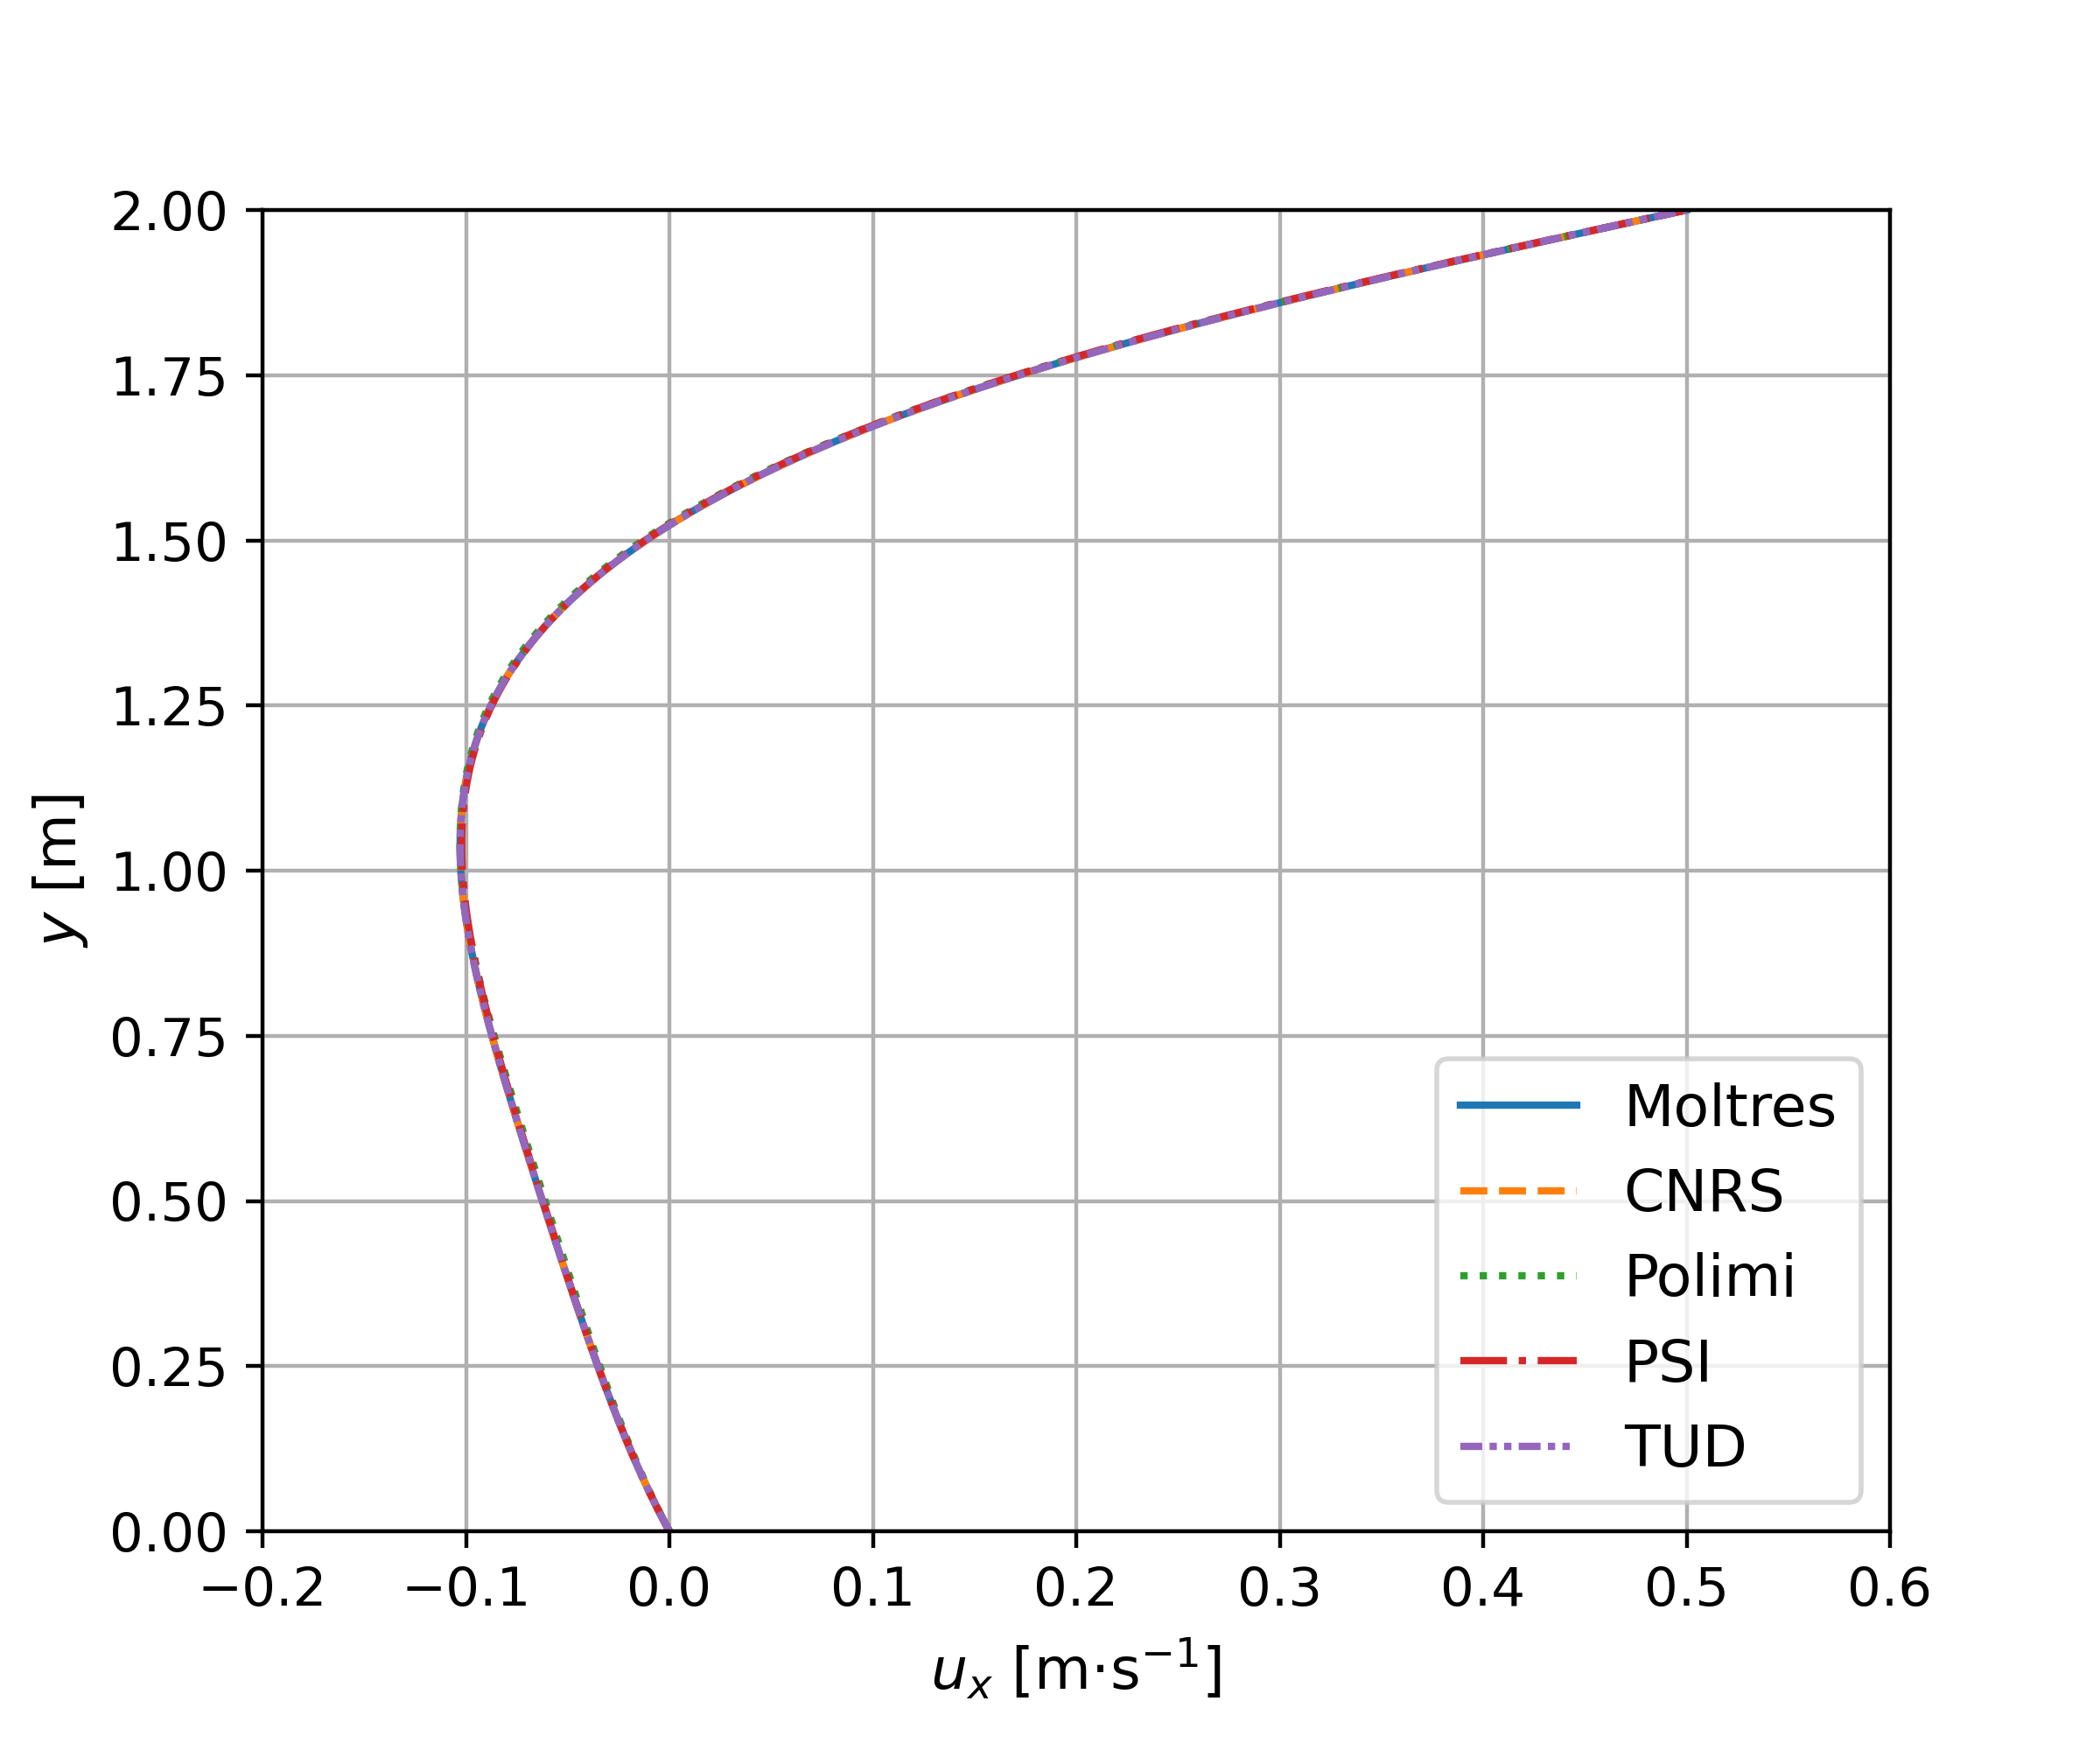
\includegraphics[width=.49\columnwidth]{0-1-vel-plot}
	\caption{Step 0.1 \textemdash\ Horizontal velocity component along BB'.}
	\label{fig:0.1}
\end{figure}
%
\begin{figure}[h]
	\centering
    \begin{subfigure}[b]{.49\textwidth}
      \centering
	  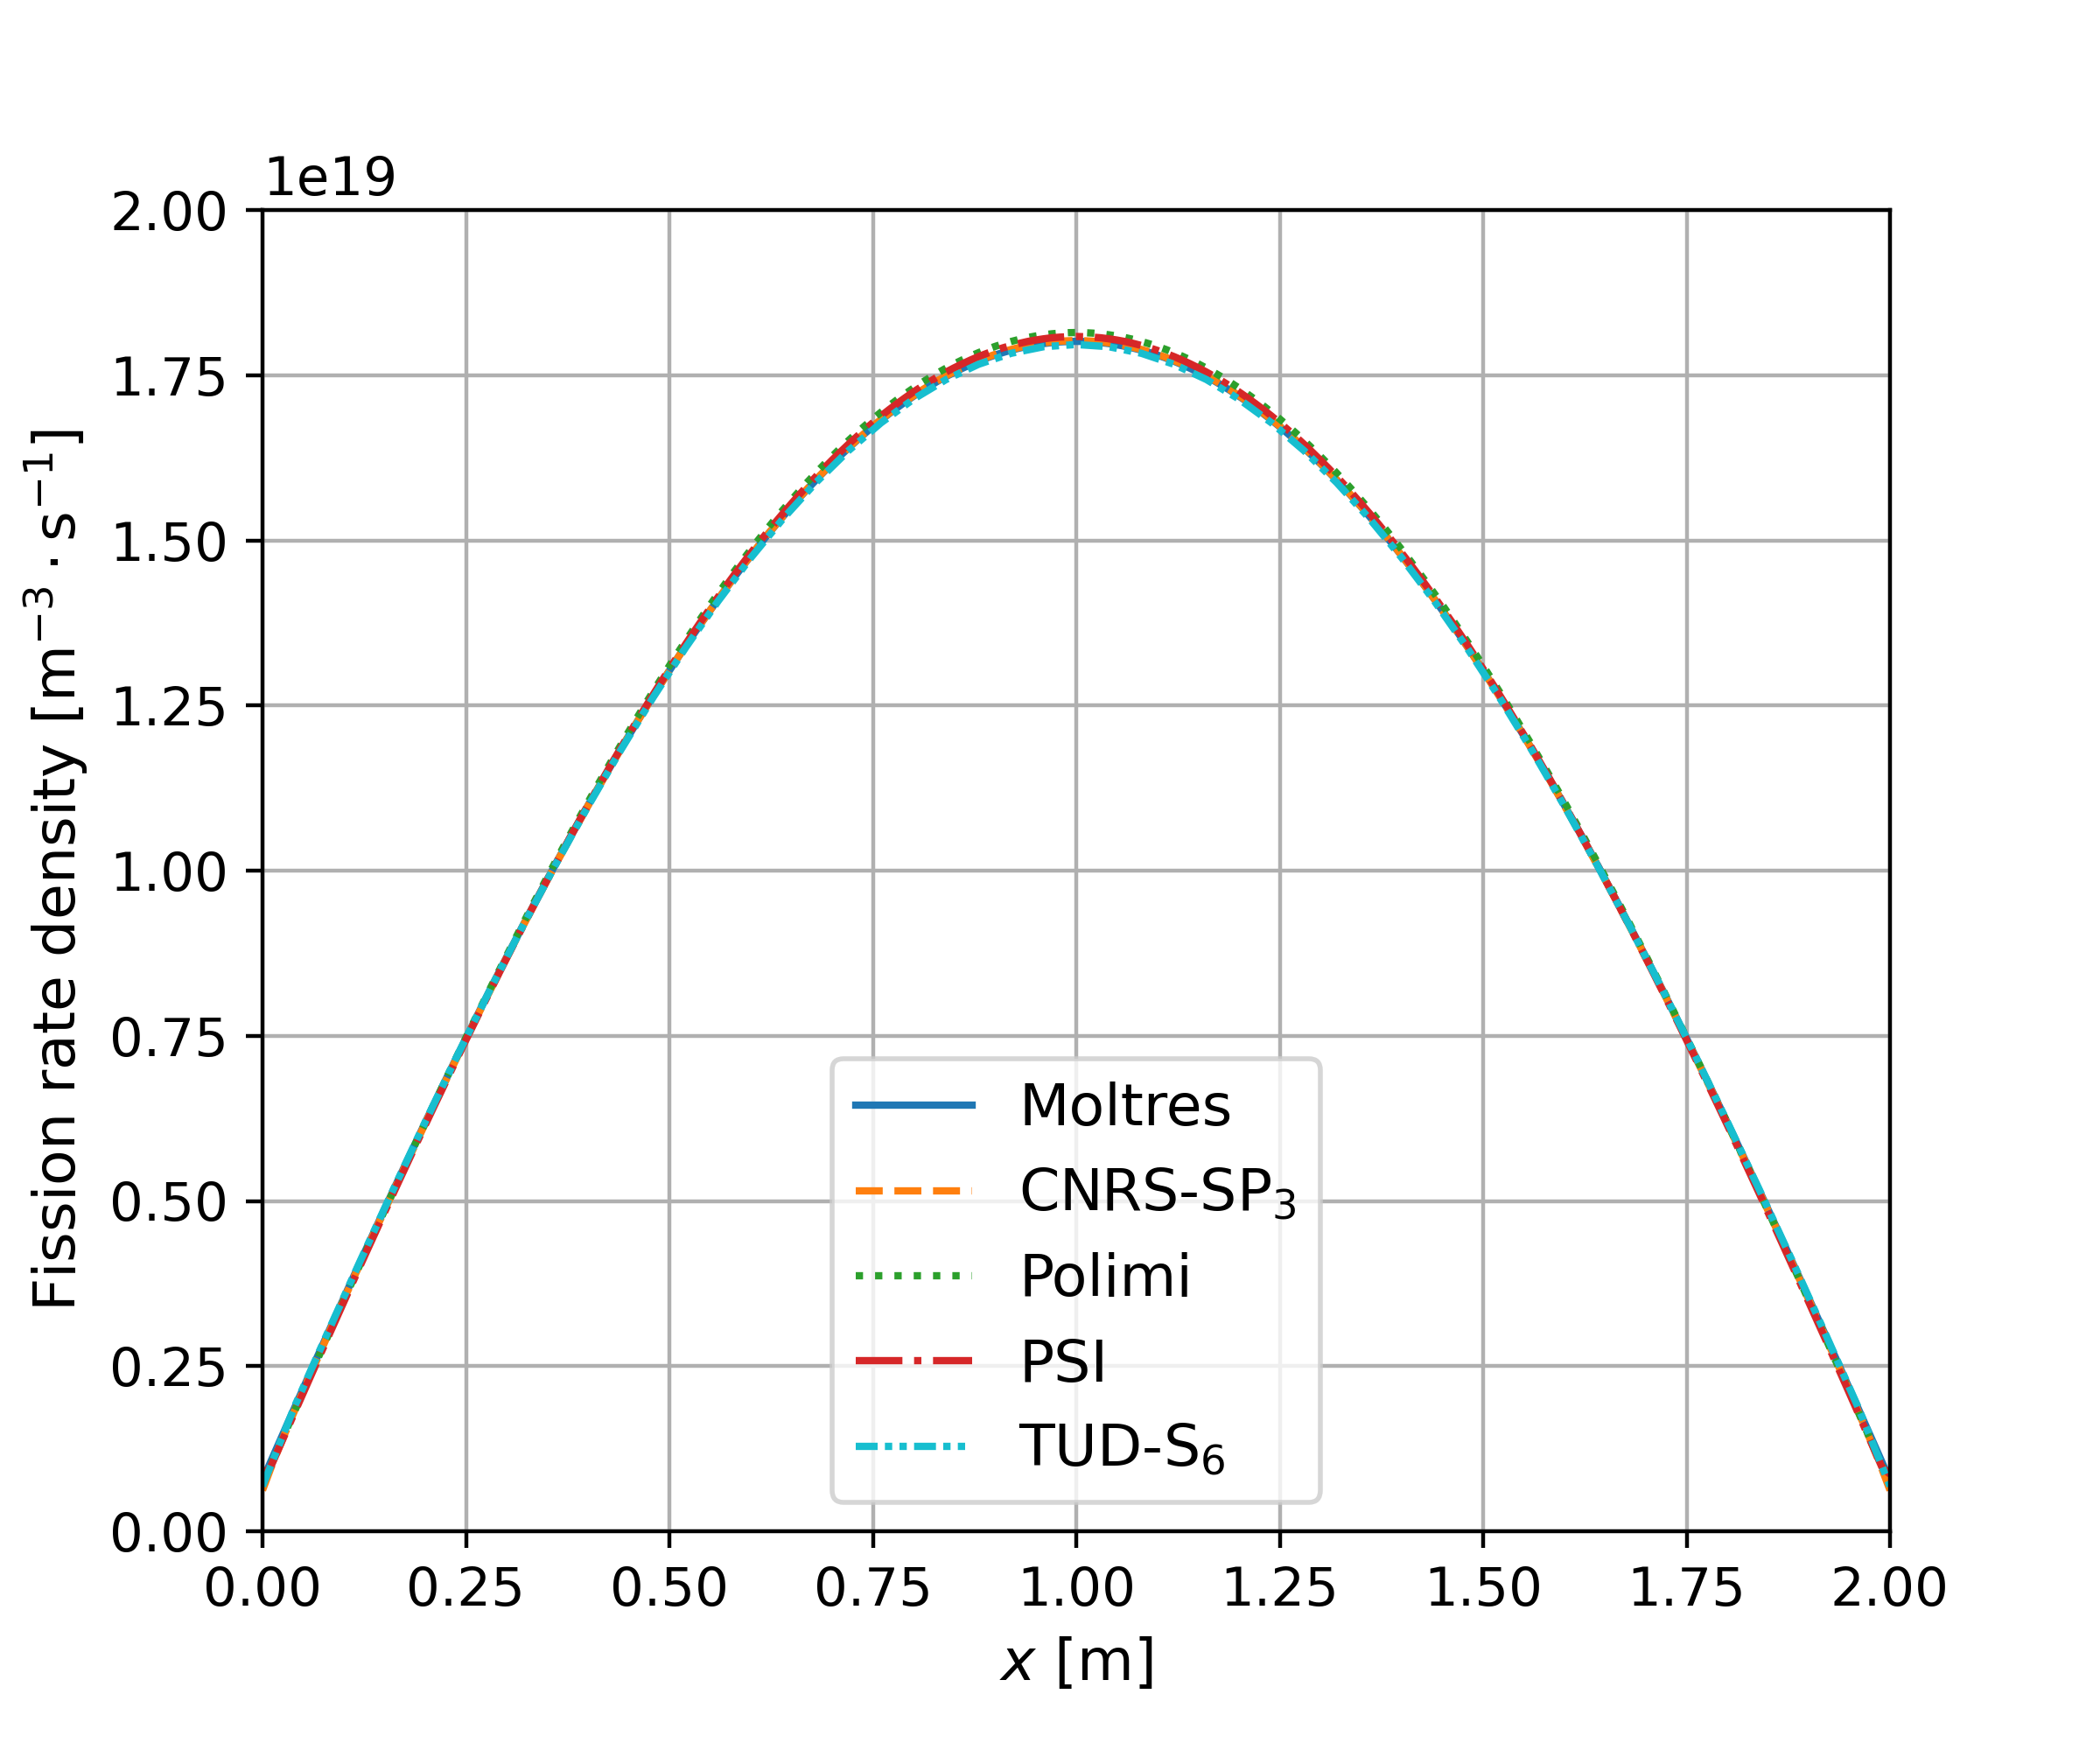
\includegraphics[width=\columnwidth]{0-2-fiss-plot}
	  \caption{Step 0.2 \textemdash\ Fission rate density along AA'.}
	  \label{fig:0.2}
    \end{subfigure}
    \hfill
    \begin{subfigure}[b]{.49\textwidth}
      \centering
	  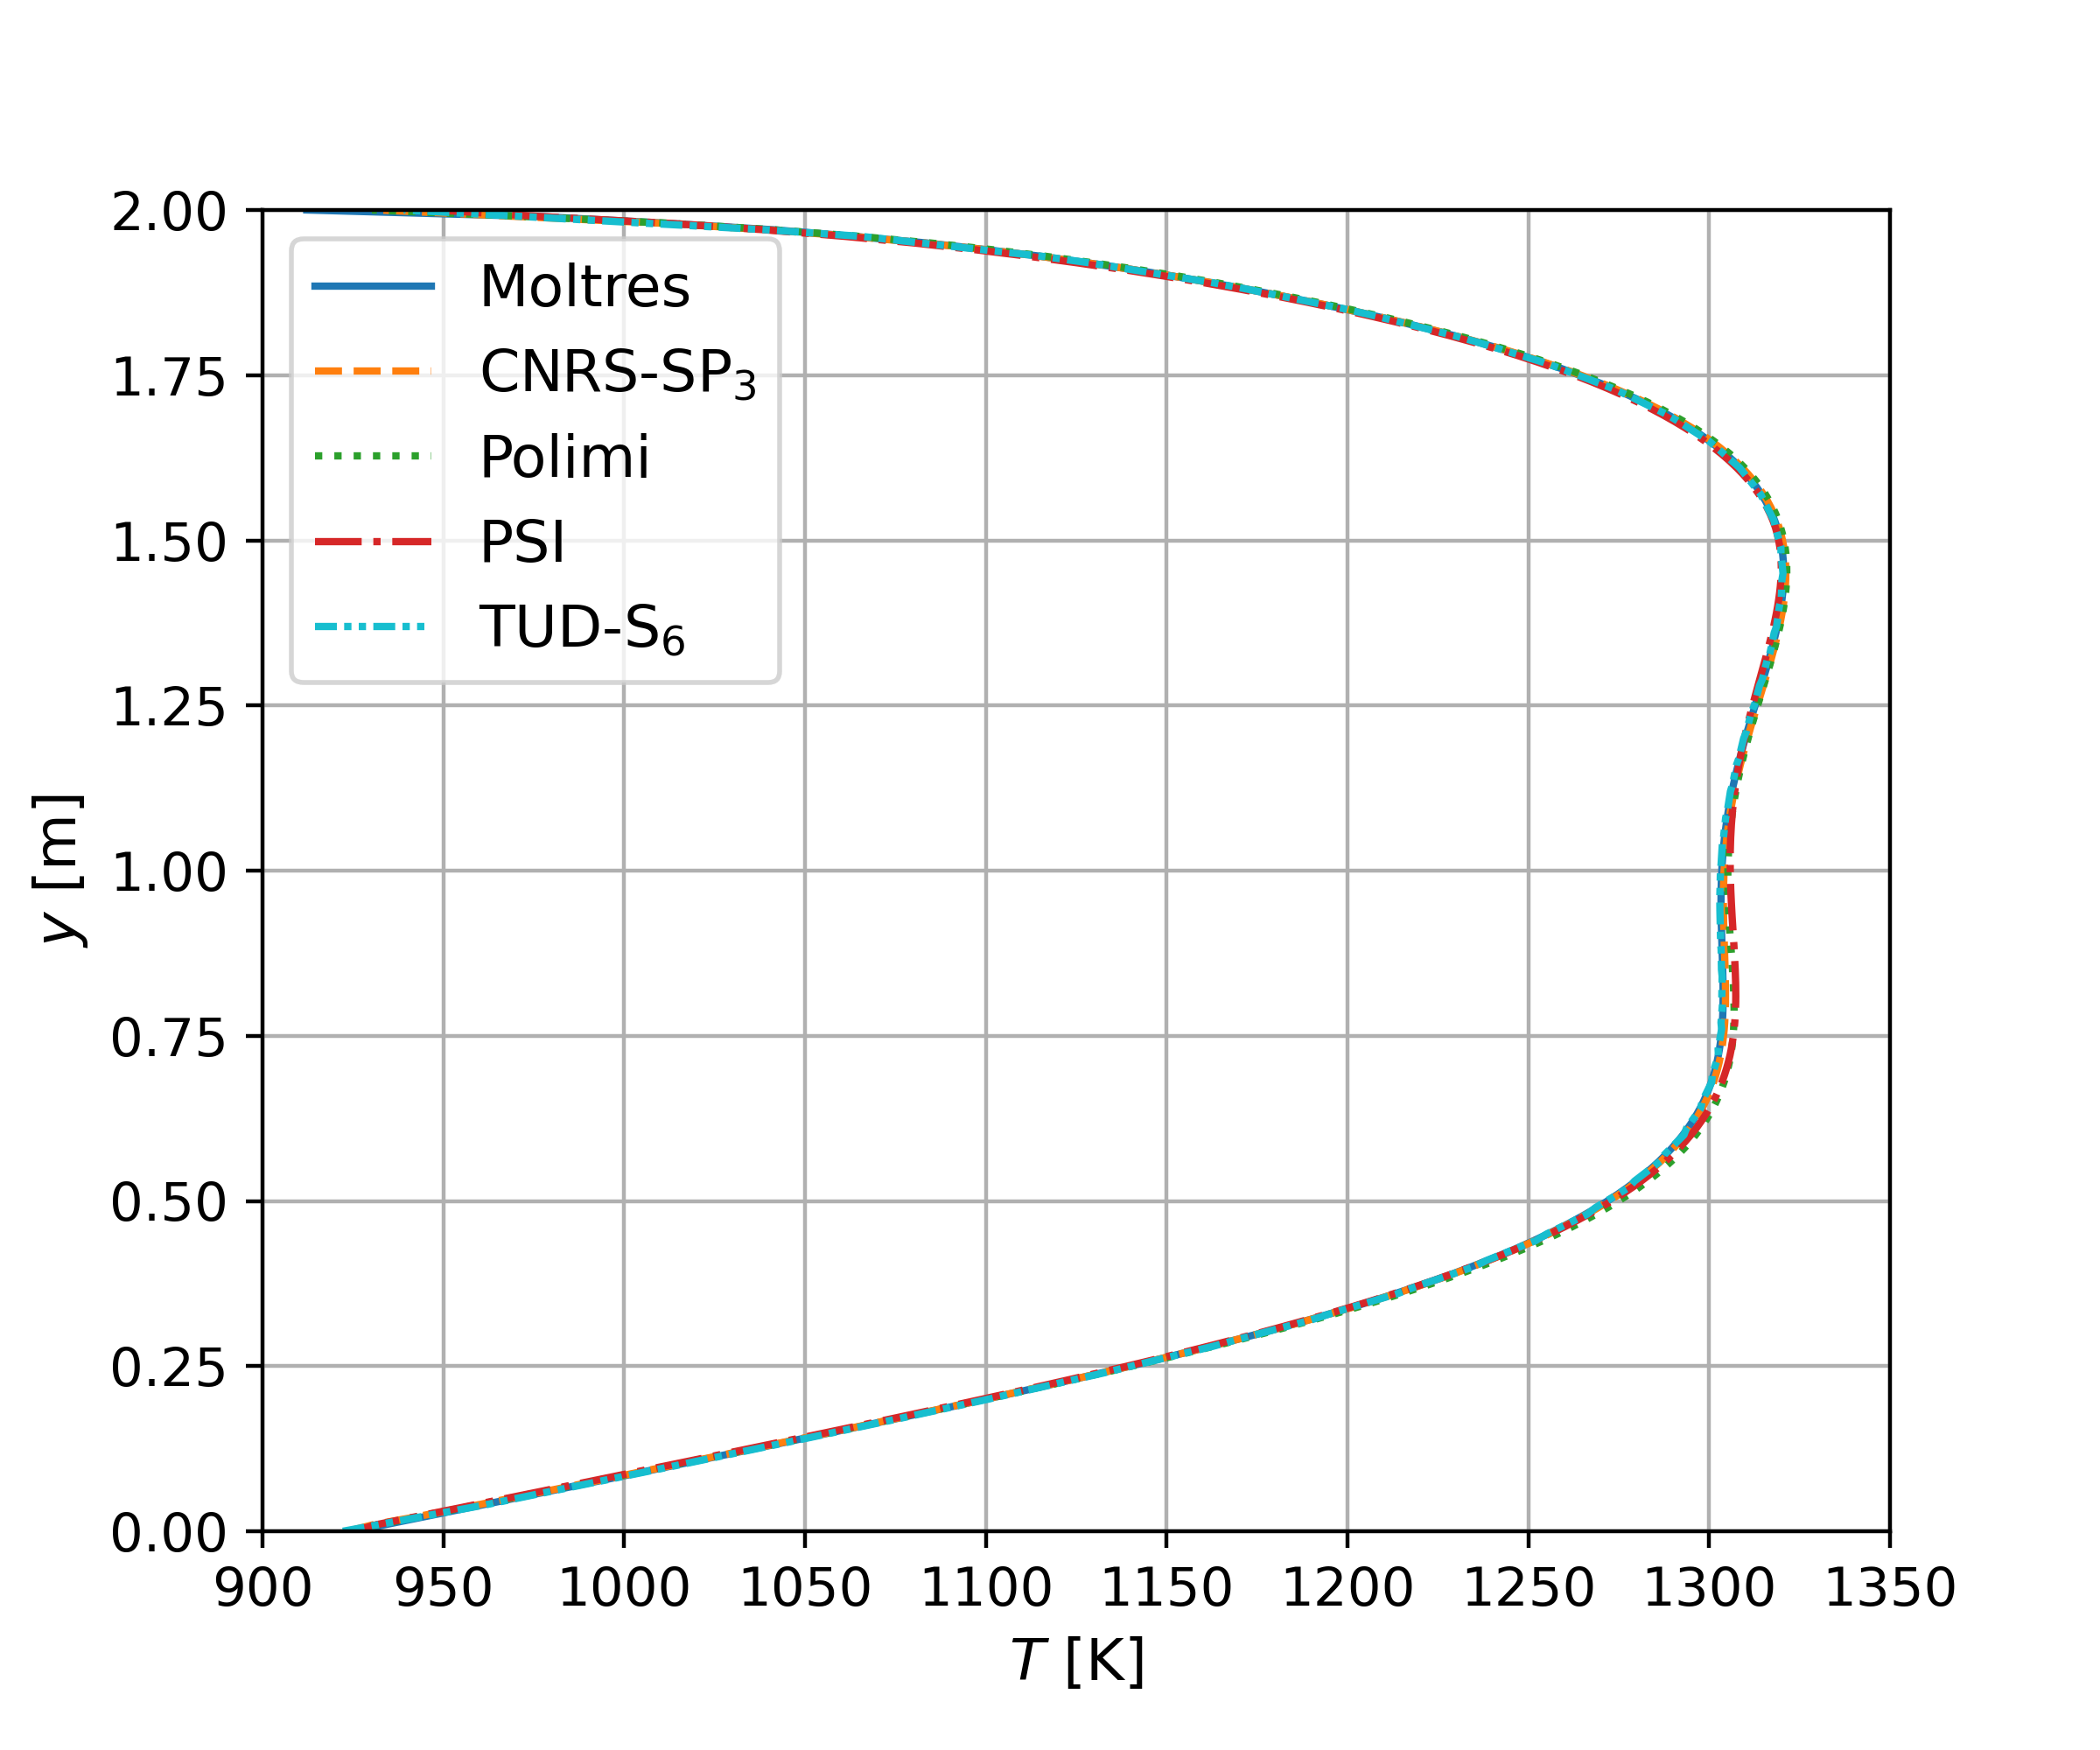
\includegraphics[width=\columnwidth]{0-3-temp-plot}
	  \caption{Step 0.3 \textemdash\ Temperature distribution along BB'.}
	  \label{fig:0.3}
    \end{subfigure}
\end{figure}
%
\FloatBarrier
%
\begin{table}[htb]
	\caption{Discrepancy values from Moltres alongside the average and standard
	deviation of the discrepancy values of the benchmark participants for Phase
	0.}
	\centering
	\small
	\begin{tabular}{l l c S S S}
		\toprule
		\multirow{2}{*}{\textbf{Step}} & \multirow{2}{*}{\textbf{Observable}} & \multirow{2}{*}{\textbf{Centerline}} & {\multirow{2}{*}{\textbf{Moltres [\%]}}} & \multicolumn{2}{c}{\textbf{Benchmark [\%]}} \\
		& & & & {Average} & {SD} \\
		\midrule
		\multirow{4}{*}{0.1} &
		\multirow{2}{*}{$u_x$} & AA' & 0.247 & 0.253 & 0.150 \\
		& & BB' & 0.266 & 0.318 & 0.102 \\
		\cmidrule{2-6}
		& \multirow{2}{*}{$u_y$} & AA' & 0.540 & 0.598 & 0.266 \\
		& & BB' & 0.468 & 0.795 & 0.421 \\
		\midrule
		{0.2} &
		{$\sum^6_g \Sigma_{f,g} \phi_g(\vec{r})$} & AA' & 0.313 & 0.285 & 0.153
		\\
		\midrule
		\multirow{2}{*}{0.3} &
		\multirow{2}{*}{$T$} & AA' & 0.090 & 0.085 & 0.031 \\
		& & BB' & 0.164 & 0.083 & 0.027\\
		\bottomrule
	\end{tabular}
	\label{table:disc0}
\end{table}

\subsubsection{Phase 0 results \& discussion}

Figures \ref{fig:0.1}, \ref{fig:0.2}, and \ref{fig:0.3} show that Moltres
accurately reproduced all three sets of results in Phase 0 for the velocity
field, fission rate density, and temperature. Table
\ref{table:disc0} reports the discrepancy values from Moltres for Phase 0 and
the corresponding average and \gls{SD} of the discrepancy values from
the benchmark participants
\cite{tiberga_results_2020}. Moltres performs very well as most discrepancy
values are either lower than or fall within one \gls{SD} of the benchmark
average discrepancies. The discrepancy value for $T$ along centerline BB' in
Step 0.3 is the only exception, with its value of 0.164\% being larger than
the benchmark average by 3 \gls{SD}.

Figure \ref{fig:0.3} shows that the $T$ distribution from Moltres is almost
identical to the corresponding distributions from CNRS-$SP_3$ and TUD-$S_6$
along most of centerline BB'. However, Figure \ref{fig:0.3-zoom} shows a
significant spread in the $T$ distributions along BB' from all software
packages near the top boundary. At $y = 2.0$ m, Moltres underpredicts the
temperature at 912.3 K compared to the benchmark participants' values which
range between 930.3 K and 948.1 K. This point on the top boundary lies directly downstream of
the velocity boundary condition discontinuity at the top-left corner.
Corner singularities are generally tricky to approximate with
continuous Galerkin methods \cite{kuhlmann_lid-driven_2018}.
The \gls{SUPG} stabilization scheme dampens numerical oscillations by
introducing pointwise artificial thermal diffusivity, which depends strongly on
the inverse of local velocity magnitude \cite{peterson_overview_2018}.
Therefore, while the \gls{SUPG} scheme effectively eliminates
spurious numerical oscillations everywhere else, it provides little damping
along the top boundary due to the relatively large non-zero velocity boundary
condition. On the other hand, the temperature values in the rest of the domain
and the average discrepancies of the other variables show that Moltres can
still accurately reproduce the expected results, and the temperature deviations
along the top boundary do not impact the overall integrity of our results.

\begin{figure}[htb]
	\centering
	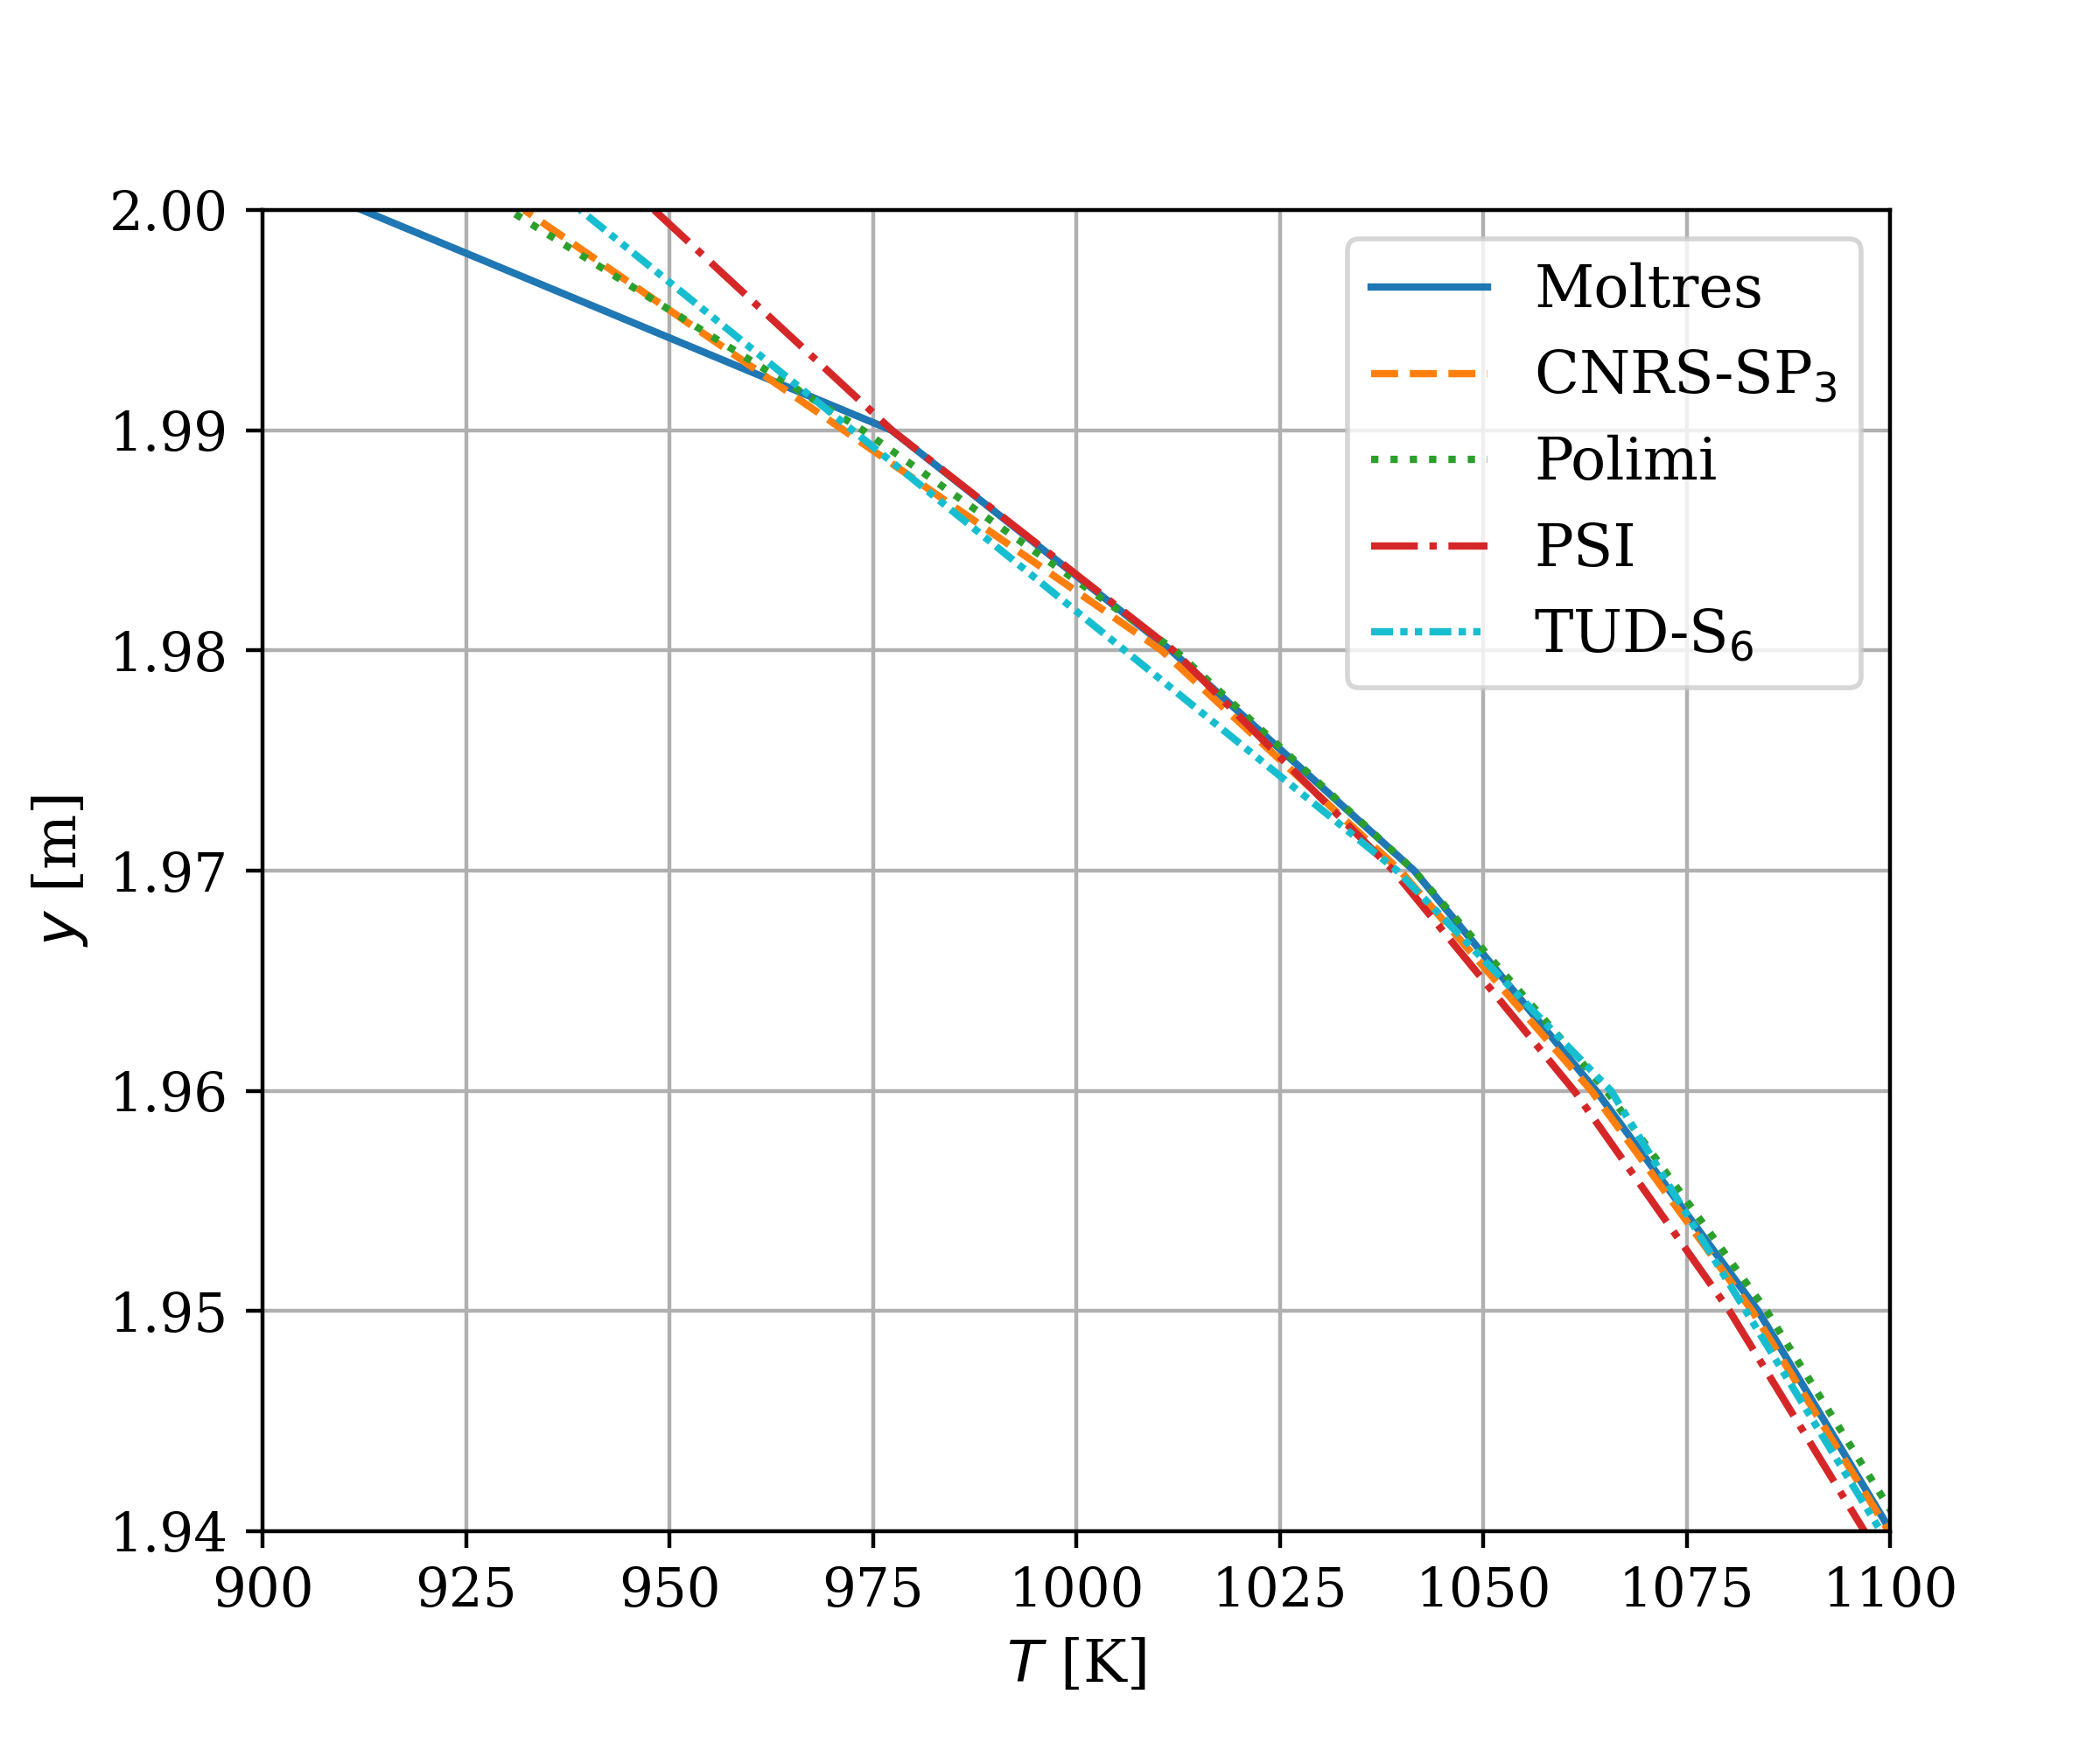
\includegraphics[width=.49\columnwidth]{0-3-temp-plot-zoom}
	\caption{Step 0.3 \textemdash\ Temperature distribution along BB' for y = 1.94 m to
	y = 2.00 m.}
	\label{fig:0.3-zoom}
\end{figure}

Lastly, we observe in table \ref{table:rho} that the reactivity $\rho$ value of
465.6 pcm from Moltres falls well within the range of $\rho$ values from the
benchmark, which range from 353.7 pcm up to 578.1 pcm. Given that Moltres 
adopts the neutron diffusion model, our $\rho$ value agrees closest to the
results from the software packages which also adopt the neutron diffusion model
or theoretically-equivalent models such as the $SP_1$ and $S_2$ neutron
transport models, namely CNRS-$SP_1$, PoliMi, PSI, and TUD-$S_2$.

\begin{table}[htb]
    \caption{Reactivity $\rho$ and change in reactivity
    $\left(\rho_a - \rho_b\right)$ values from Steps 0.2, 1.1,
    1.2, and 1.3. All units are in pcm.}
    \centering
    \small
    \setlength\tabcolsep{2pt}
    \begin{tabular}{l S S S S}
        \toprule
        \multirow{2}{*}{\textbf{Software}} & {\textbf{Step 0.2}} &
        {\textbf{Step 1.1}} & {\textbf{Step 1.2}} & {\textbf{Step 1.3}} \\
        & {$\rho_{s_{0.2}}$}
        & {$\rho_{s_{1.1}} - \rho_{s_{0.2}}$}
        & {$\rho_{s_{1.2}} - \rho_{s_{1.1}}$}
        & {$\rho_{s_{1.3}} - \rho_{s_{0.2}}$} \\
        \midrule
        Moltres     & 465.6 & -62.7 & -1142.2 & -1207.7 \\
        CNRS-$SP_1$ & 411.3 & -62.5 & -1152.0 & -1220.5 \\
        CNRS-$SP_3$ & 353.7 & -62.6 & -1152.7 & -1220.7 \\
        PoliMi      & 421.2 & -62.0 & -1161.0 & -1227.0 \\
        PSI         & 411.7 & -63.0 & -1154.8 & -1219.6 \\
        TUD-$S_2$   & 482.6 & -62.0 & -1145.2 & -1208.5 \\
        TUD-$S_6$   & 578.1 & -60.7 & -1122.0 & -1184.4 \\
        \bottomrule
    \end{tabular}
    \label{table:rho}
\end{table}

\FloatBarrier

\subsubsection{Phase 1 results \& discussion}

Table \ref{table:disc1} shows the discrepancy values from Moltres relative to
the average and \gls{SD} of the benchmark participants for Steps 1.1, 1.2, and
1.3 and the corresponding average discrepancy values from the benchmark
\cite{tiberga_results_2020}. The subsequent subsections discuss the results
for each benchmark step in Phase 1.
%
\begin{table}[htb]
	\caption{Discrepancy values from Moltres alongside the average and standard
	deviation of the discrepancy values of the benchmark participants for Phase
	1.}
	\centering
	\small
	\begin{tabular}{l l c S S S}
		\toprule
		\multirow{2}{*}{\textbf{Step}} & \multirow{2}{*}{\textbf{Observable}} & \multirow{2}{*}{\textbf{Centerline}} & {\multirow{2}{*}{\textbf{Moltres [\%]}}} & \multicolumn{2}{c}{\textbf{Benchmark [\%]}} \\
		& & & & {Average} & {SD} \\
		\midrule
		\multirow{2}{*}{1.1} &
		\multirow{2}{*}{$\sum_i \lambda_i C_i$} & AA' & 0.603 & 0.346 & 0.166
		\\
		& & BB' & 0.327 & 0.294 & 0.153 \\
		\midrule
		\multirow{4}{*}{1.2} &
		\multirow{2}{*}{$T$} & AA' & 0.076 & 0.095 & 0.015 \\
		& & BB' & 0.179 & 0.089 & 0.012 \\
		\cmidrule{2-6}
		& \multirow{2}{*}{\footnotesize $\Delta\left[\sum^6_g \Sigma_{f,g} \phi_g(\vec{r})
		\right]_{s_{1.2}-s_{0.2}}$} & AA' & 1.110 & 1.576 & 0.564 \\
		& & BB' & 1.089 & 1.133 & 0.392 \\
		\midrule
		\multirow{7}{*}{1.3} &
		{$u_x$} & AA' & 0.123 & 0.691 & 0.566 \\
		\cmidrule{2-6}
		& \multirow{2}{*}{$u_y$} & AA' & 0.237 & 0.329 & 0.131 \\
		& & BB' & 0.238 & 0.356 & 0.217 \\
		\cmidrule{2-6}
		& \multirow{2}{*}{$T$} & AA' & 0.064 & 0.057 & 0.023 \\
		& & BB' & 0.070 & 0.080 & 0.024 \\
		\cmidrule{2-6}
		& \multirow{2}{*}{$\sum_i \lambda_i C_i$} & AA' & 1.043 & 0.460 & 0.190
		\\
		& & BB' & 0.462 & 1.194 & 0.178 \\
		\bottomrule
	\end{tabular}
	\label{table:disc1}
\end{table}

\paragraph{Step 1.1: Circulating fuel}

Figure \ref{fig:1.1} shows good qualitative agreement in the delayed neutron
source distribution along BB' among Moltres and the benchmark participants.
From Table \ref{table:disc1}, Moltres reports discrepancies of 0.603\% and
0.327\% along the centerlines AA' and BB', respectively. Both values are
within two and one \gls{SD}, respectively, of the average discrepancies of the
benchmark participants (0.346\% and 0.294\%).
In Table \ref{table:rho}, we observe that the change in
$\rho$ relative to Step 0.2 is $-62.7$ pcm for Moltres, and this value is
consistent with the $-63.0$ to $-62.0$ pcm range that most of the benchmark
participants' values fall in.
%
\begin{figure}[htb]
	\centering
    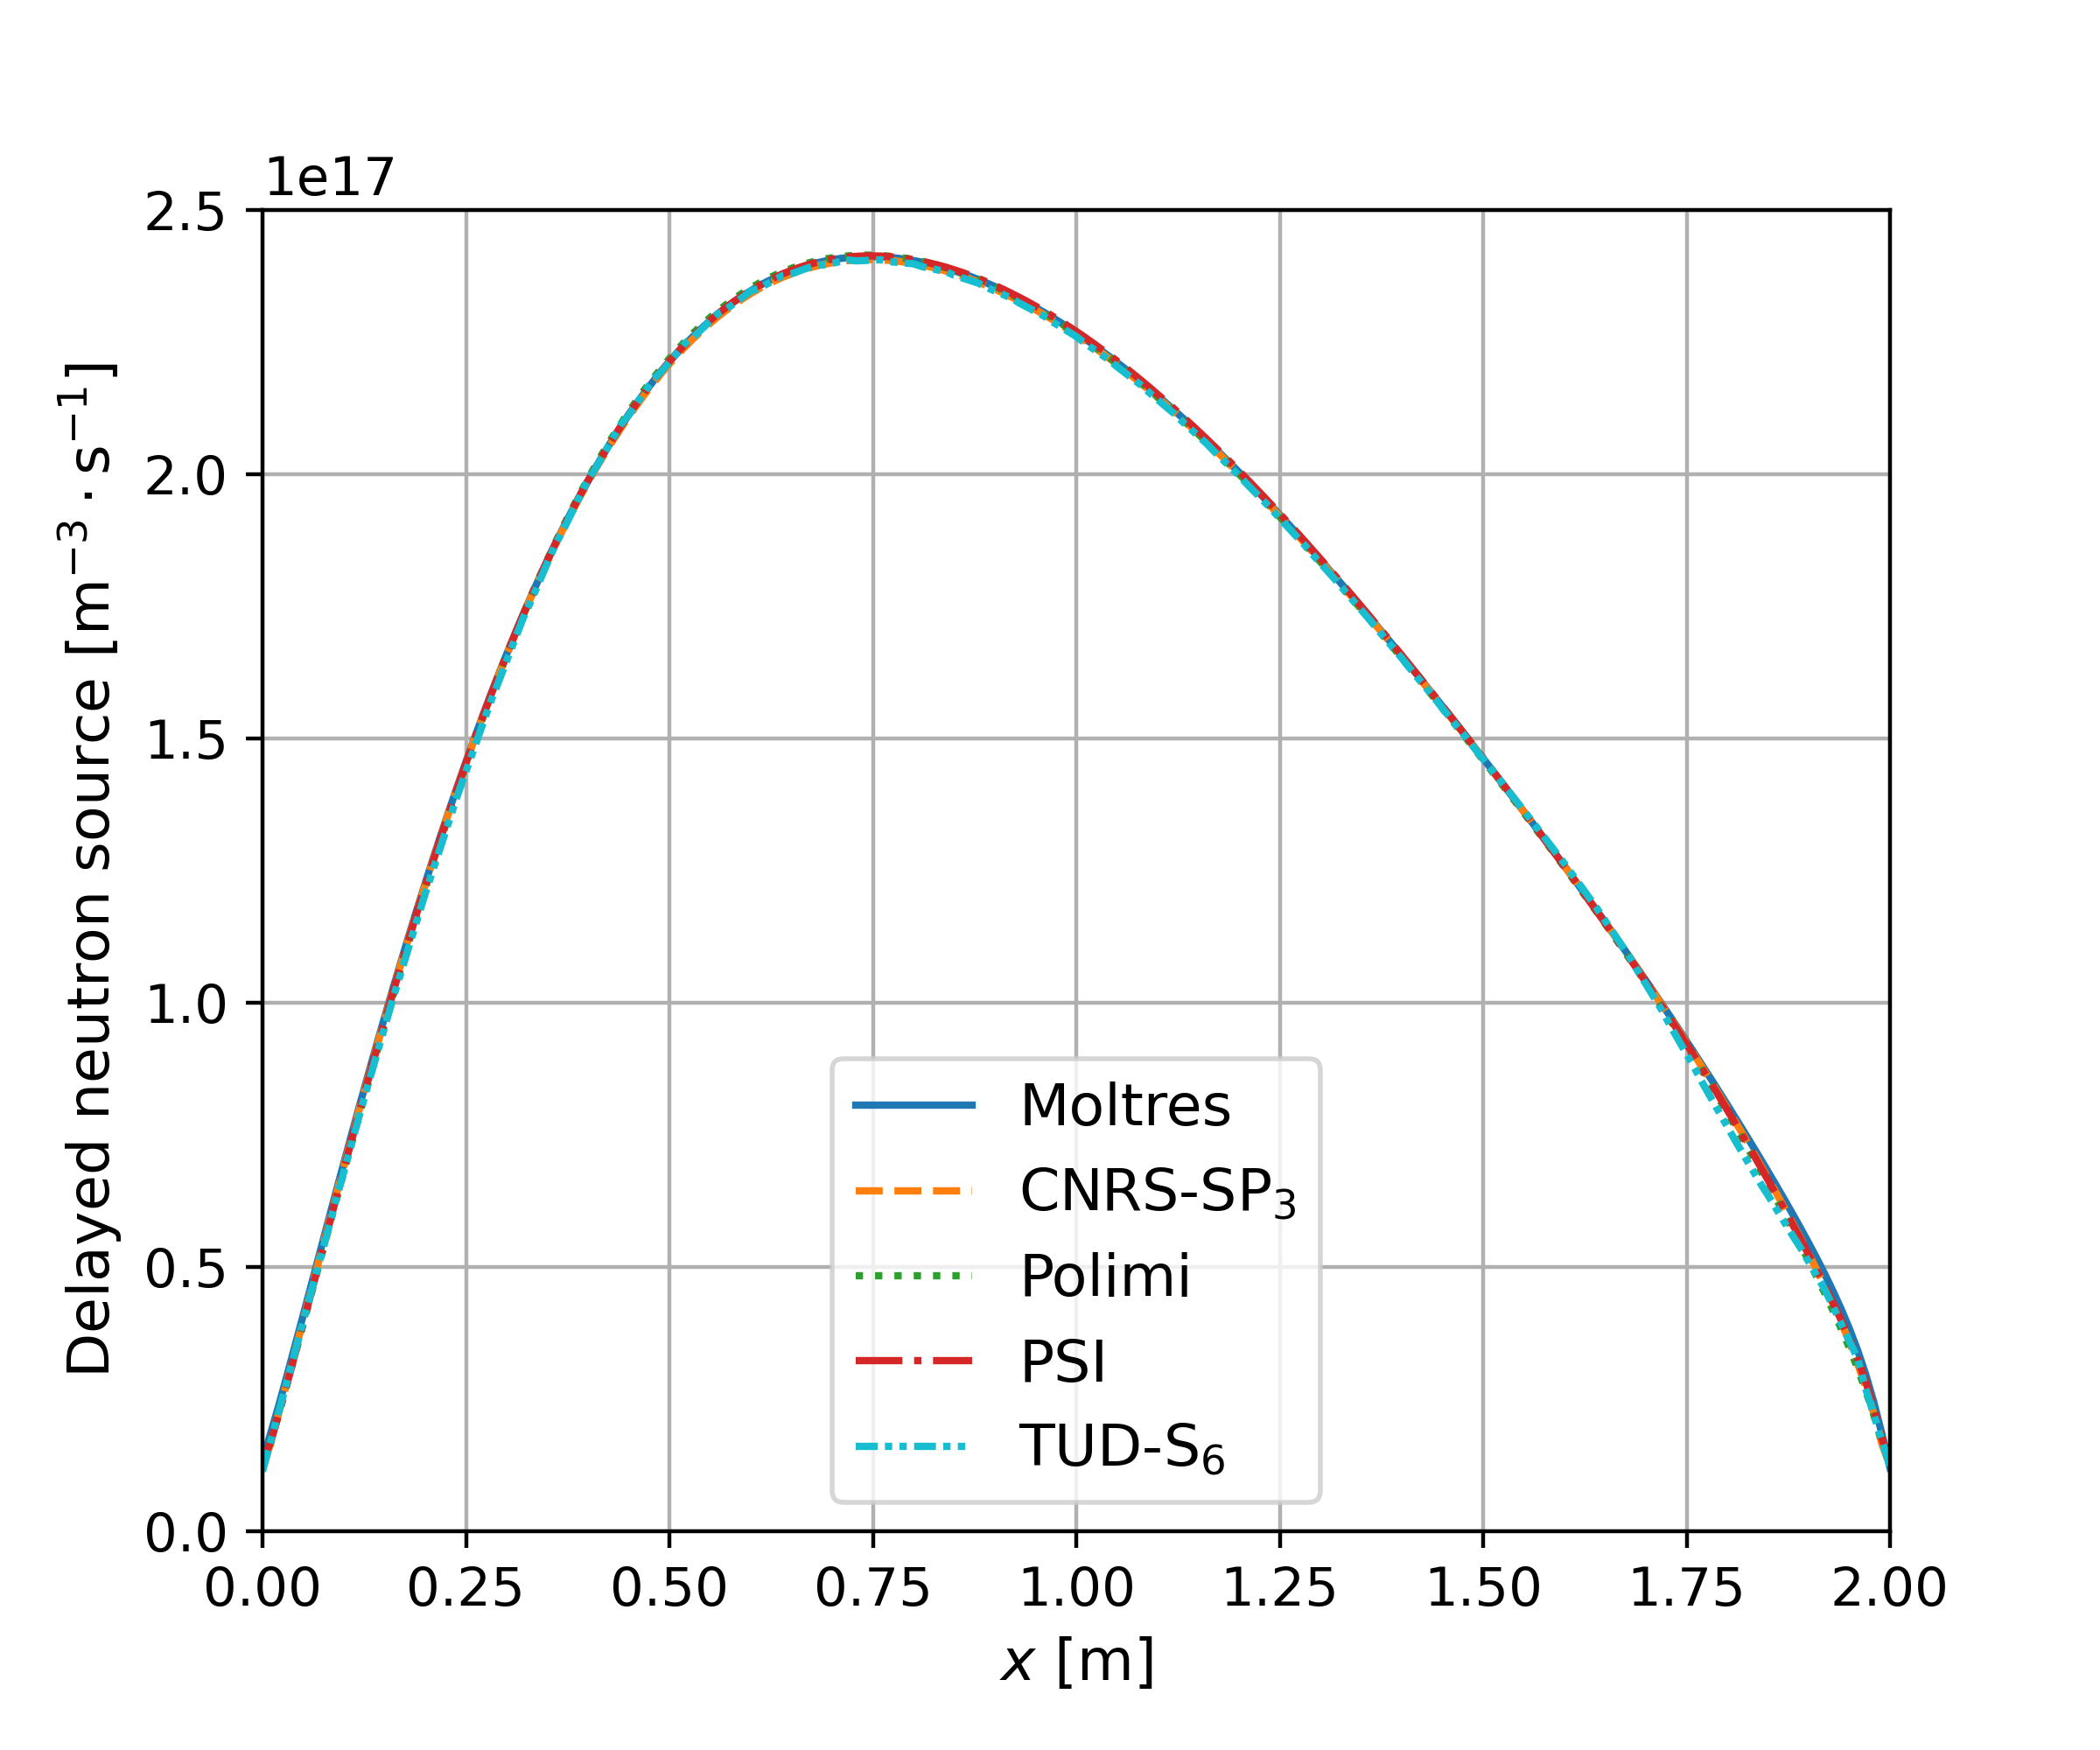
\includegraphics[width=.49\columnwidth]{1-1-dnp-x-plot}
    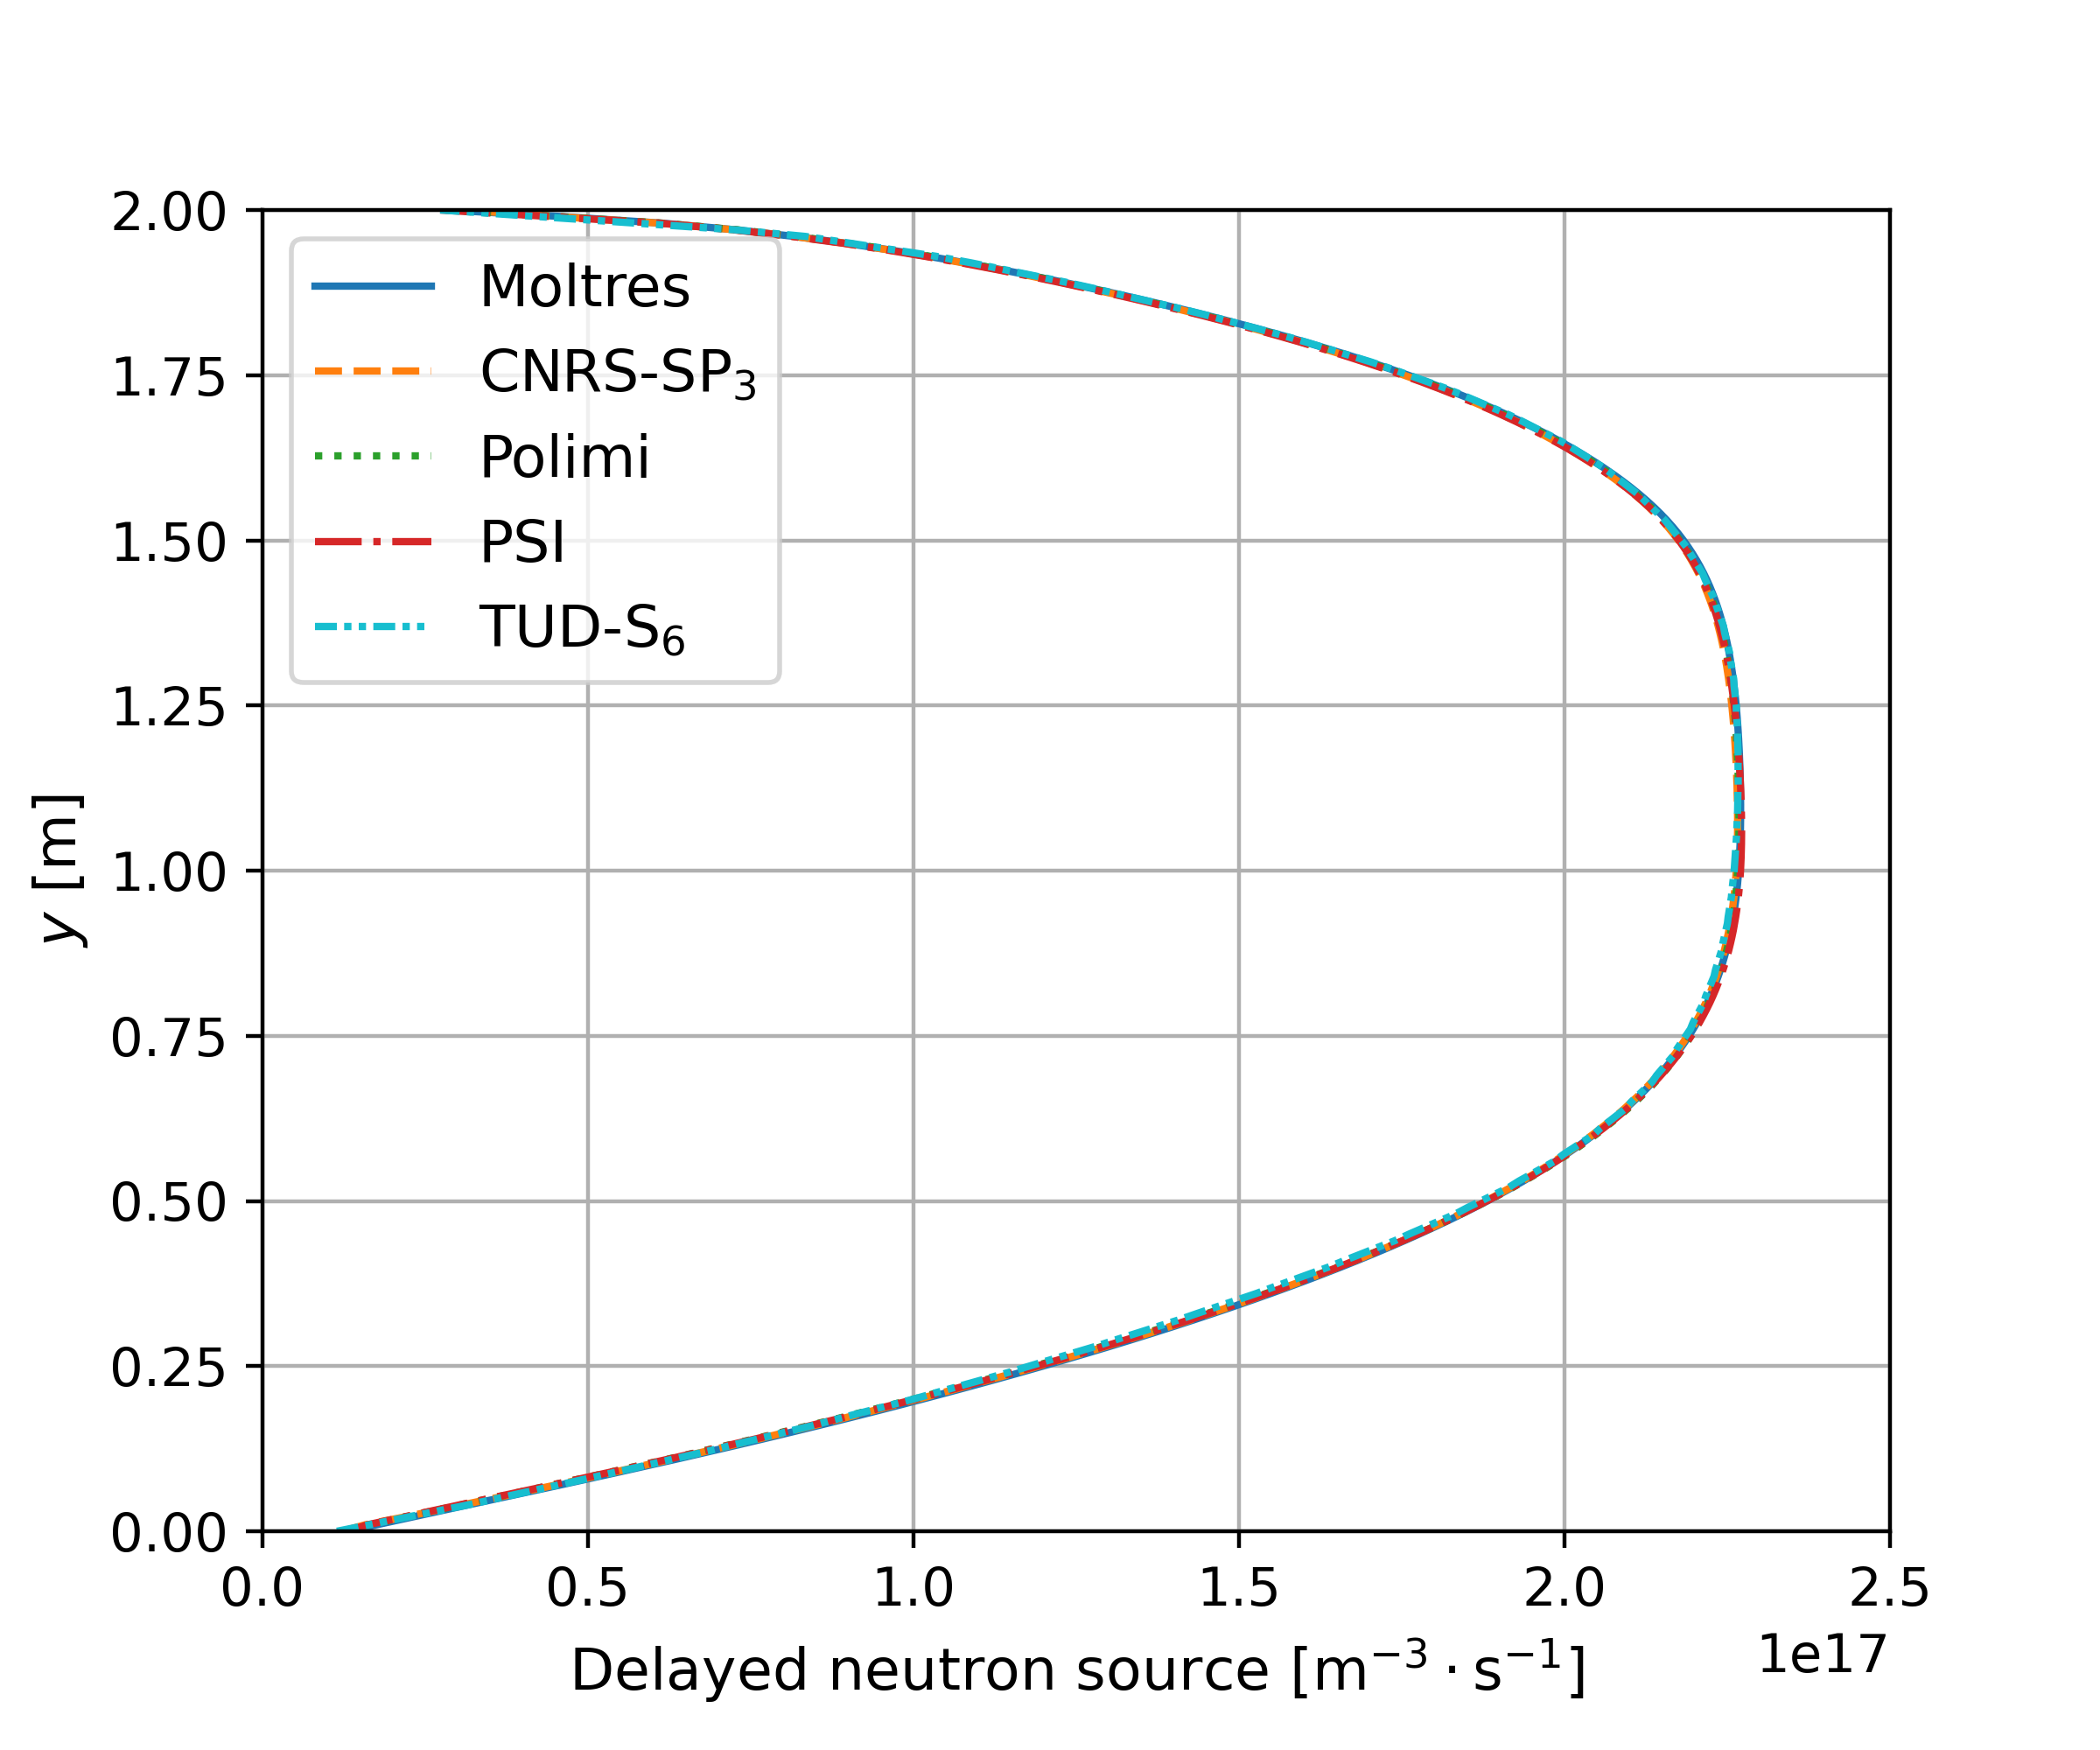
\includegraphics[width=.49\columnwidth]{1-1-dnp-y-plot}
	\caption{Step 1.1 \textemdash\ Delayed neutron source along AA' (top) and BB'
	(bottom).}
	\label{fig:1.1}
\end{figure}
%
\begin{figure}[htb]
	\centering
	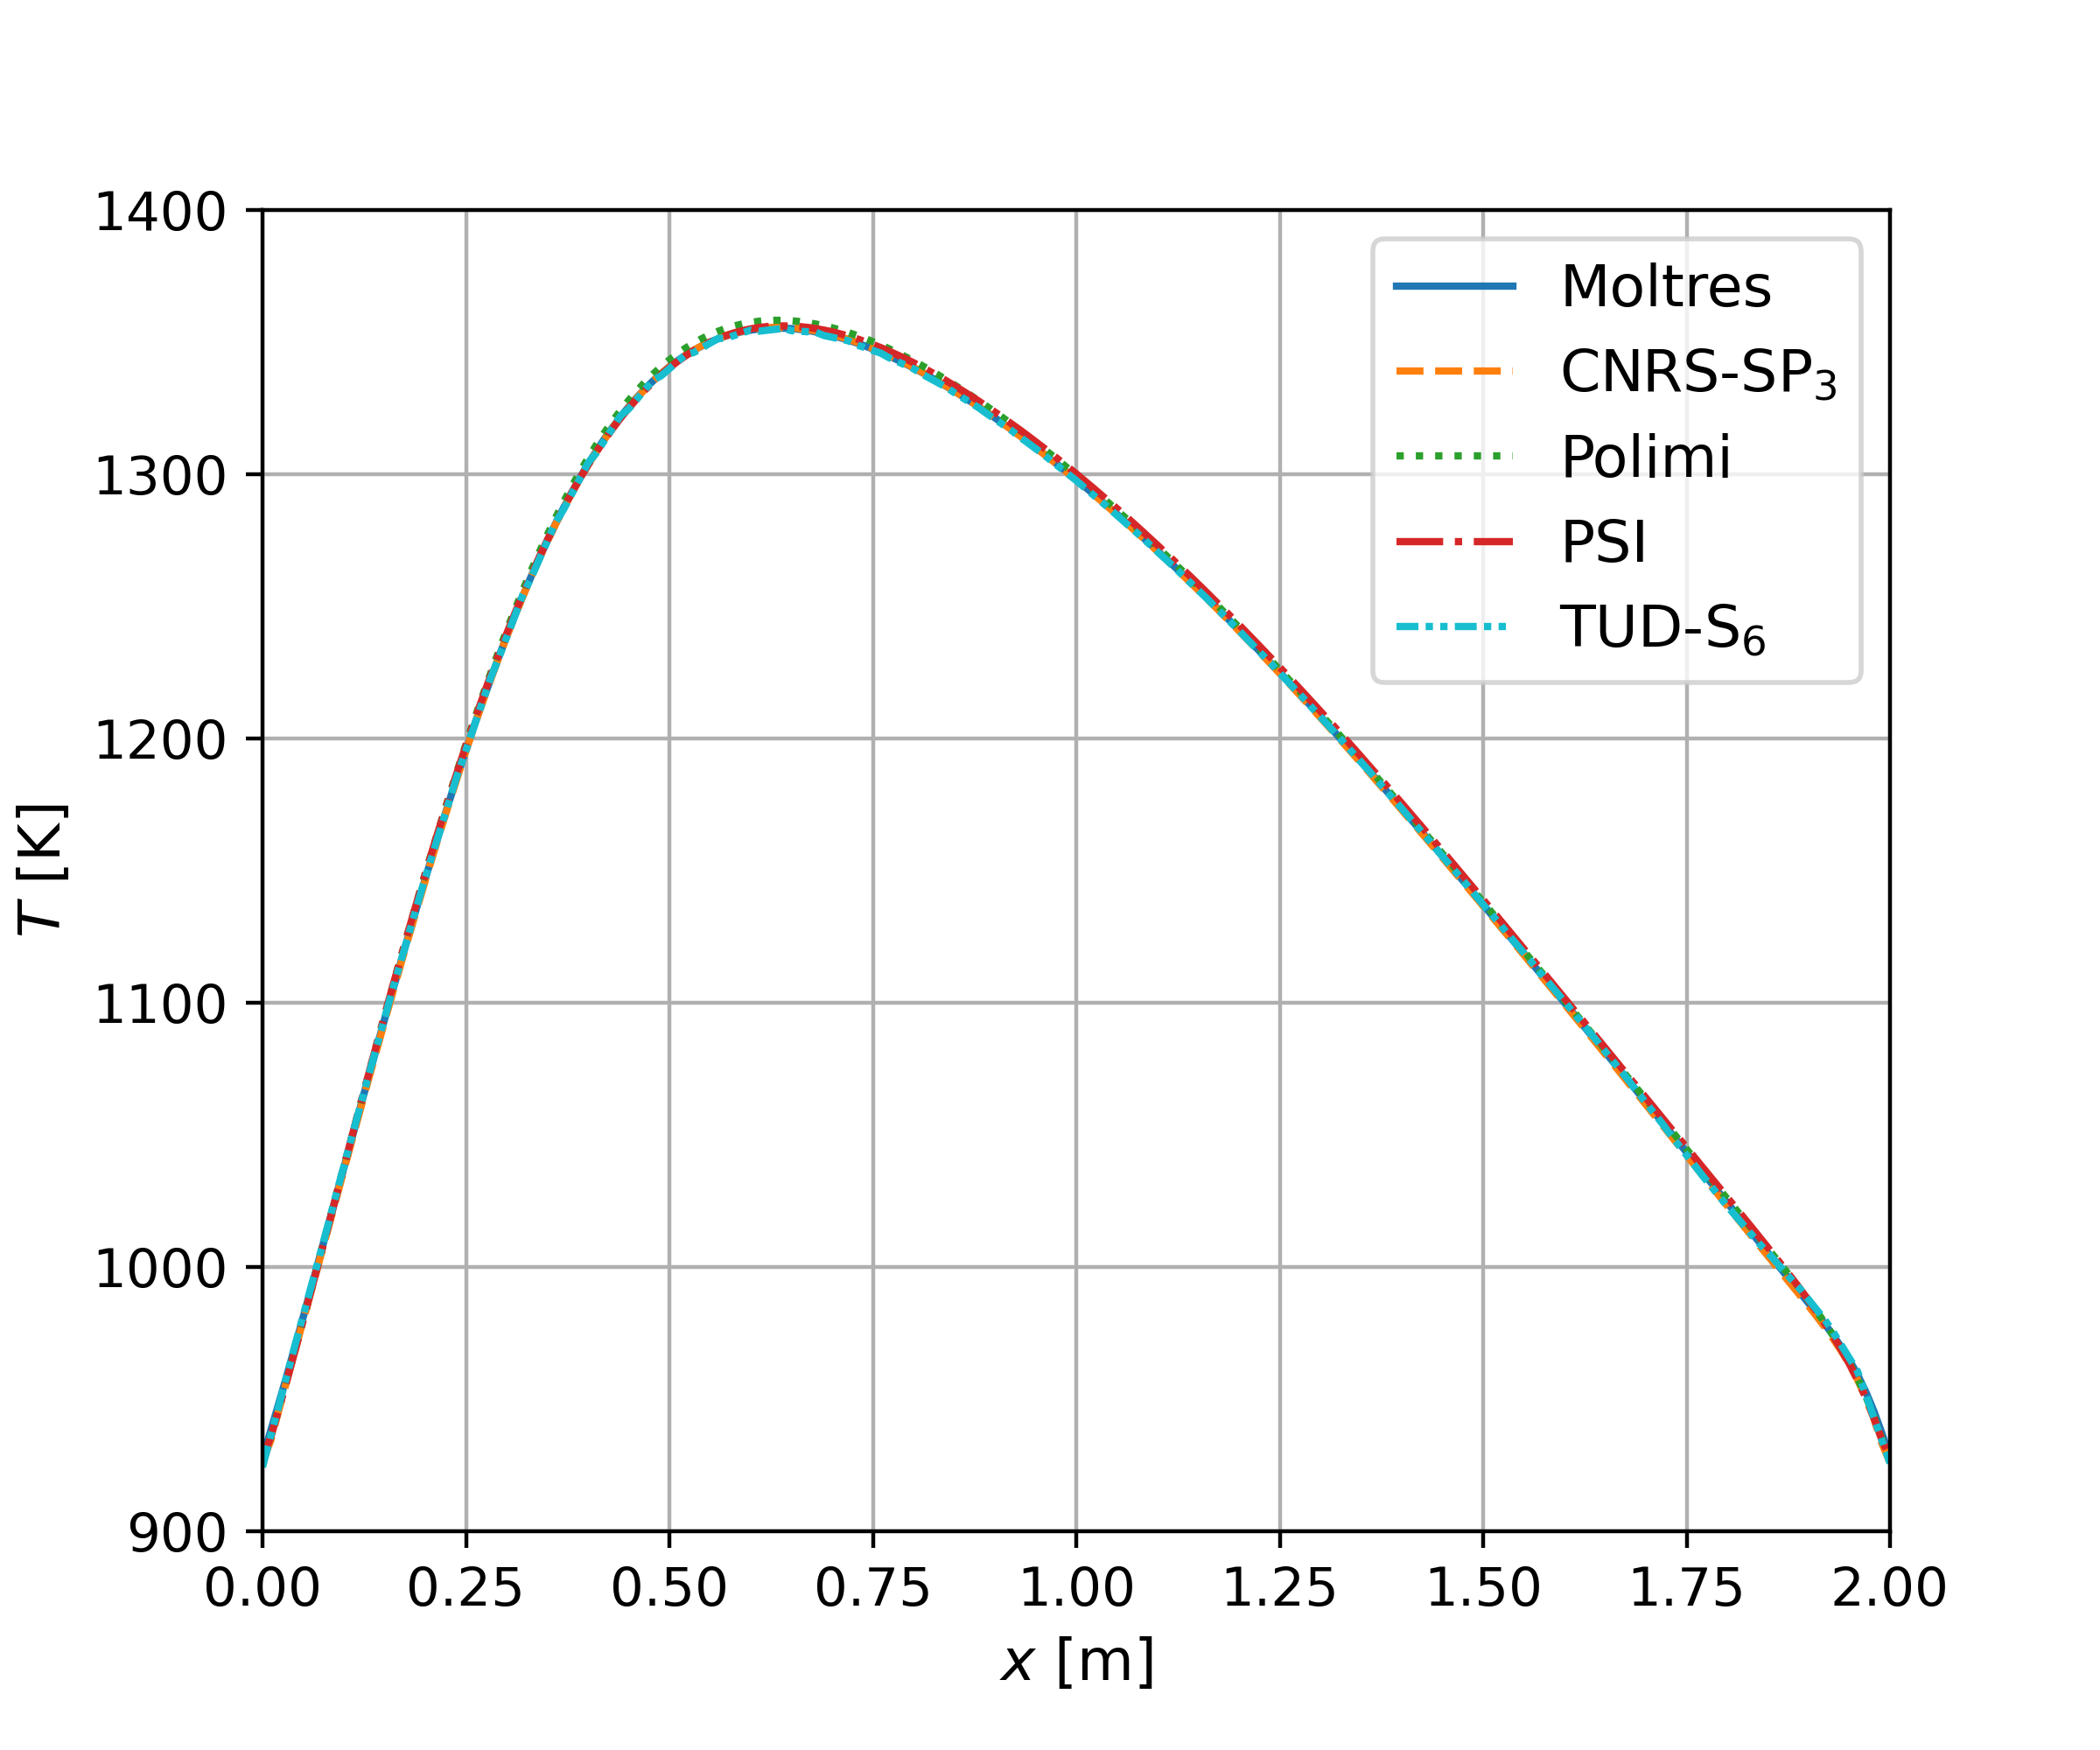
\includegraphics[width=.49\columnwidth]{1-2-temp-plot}
	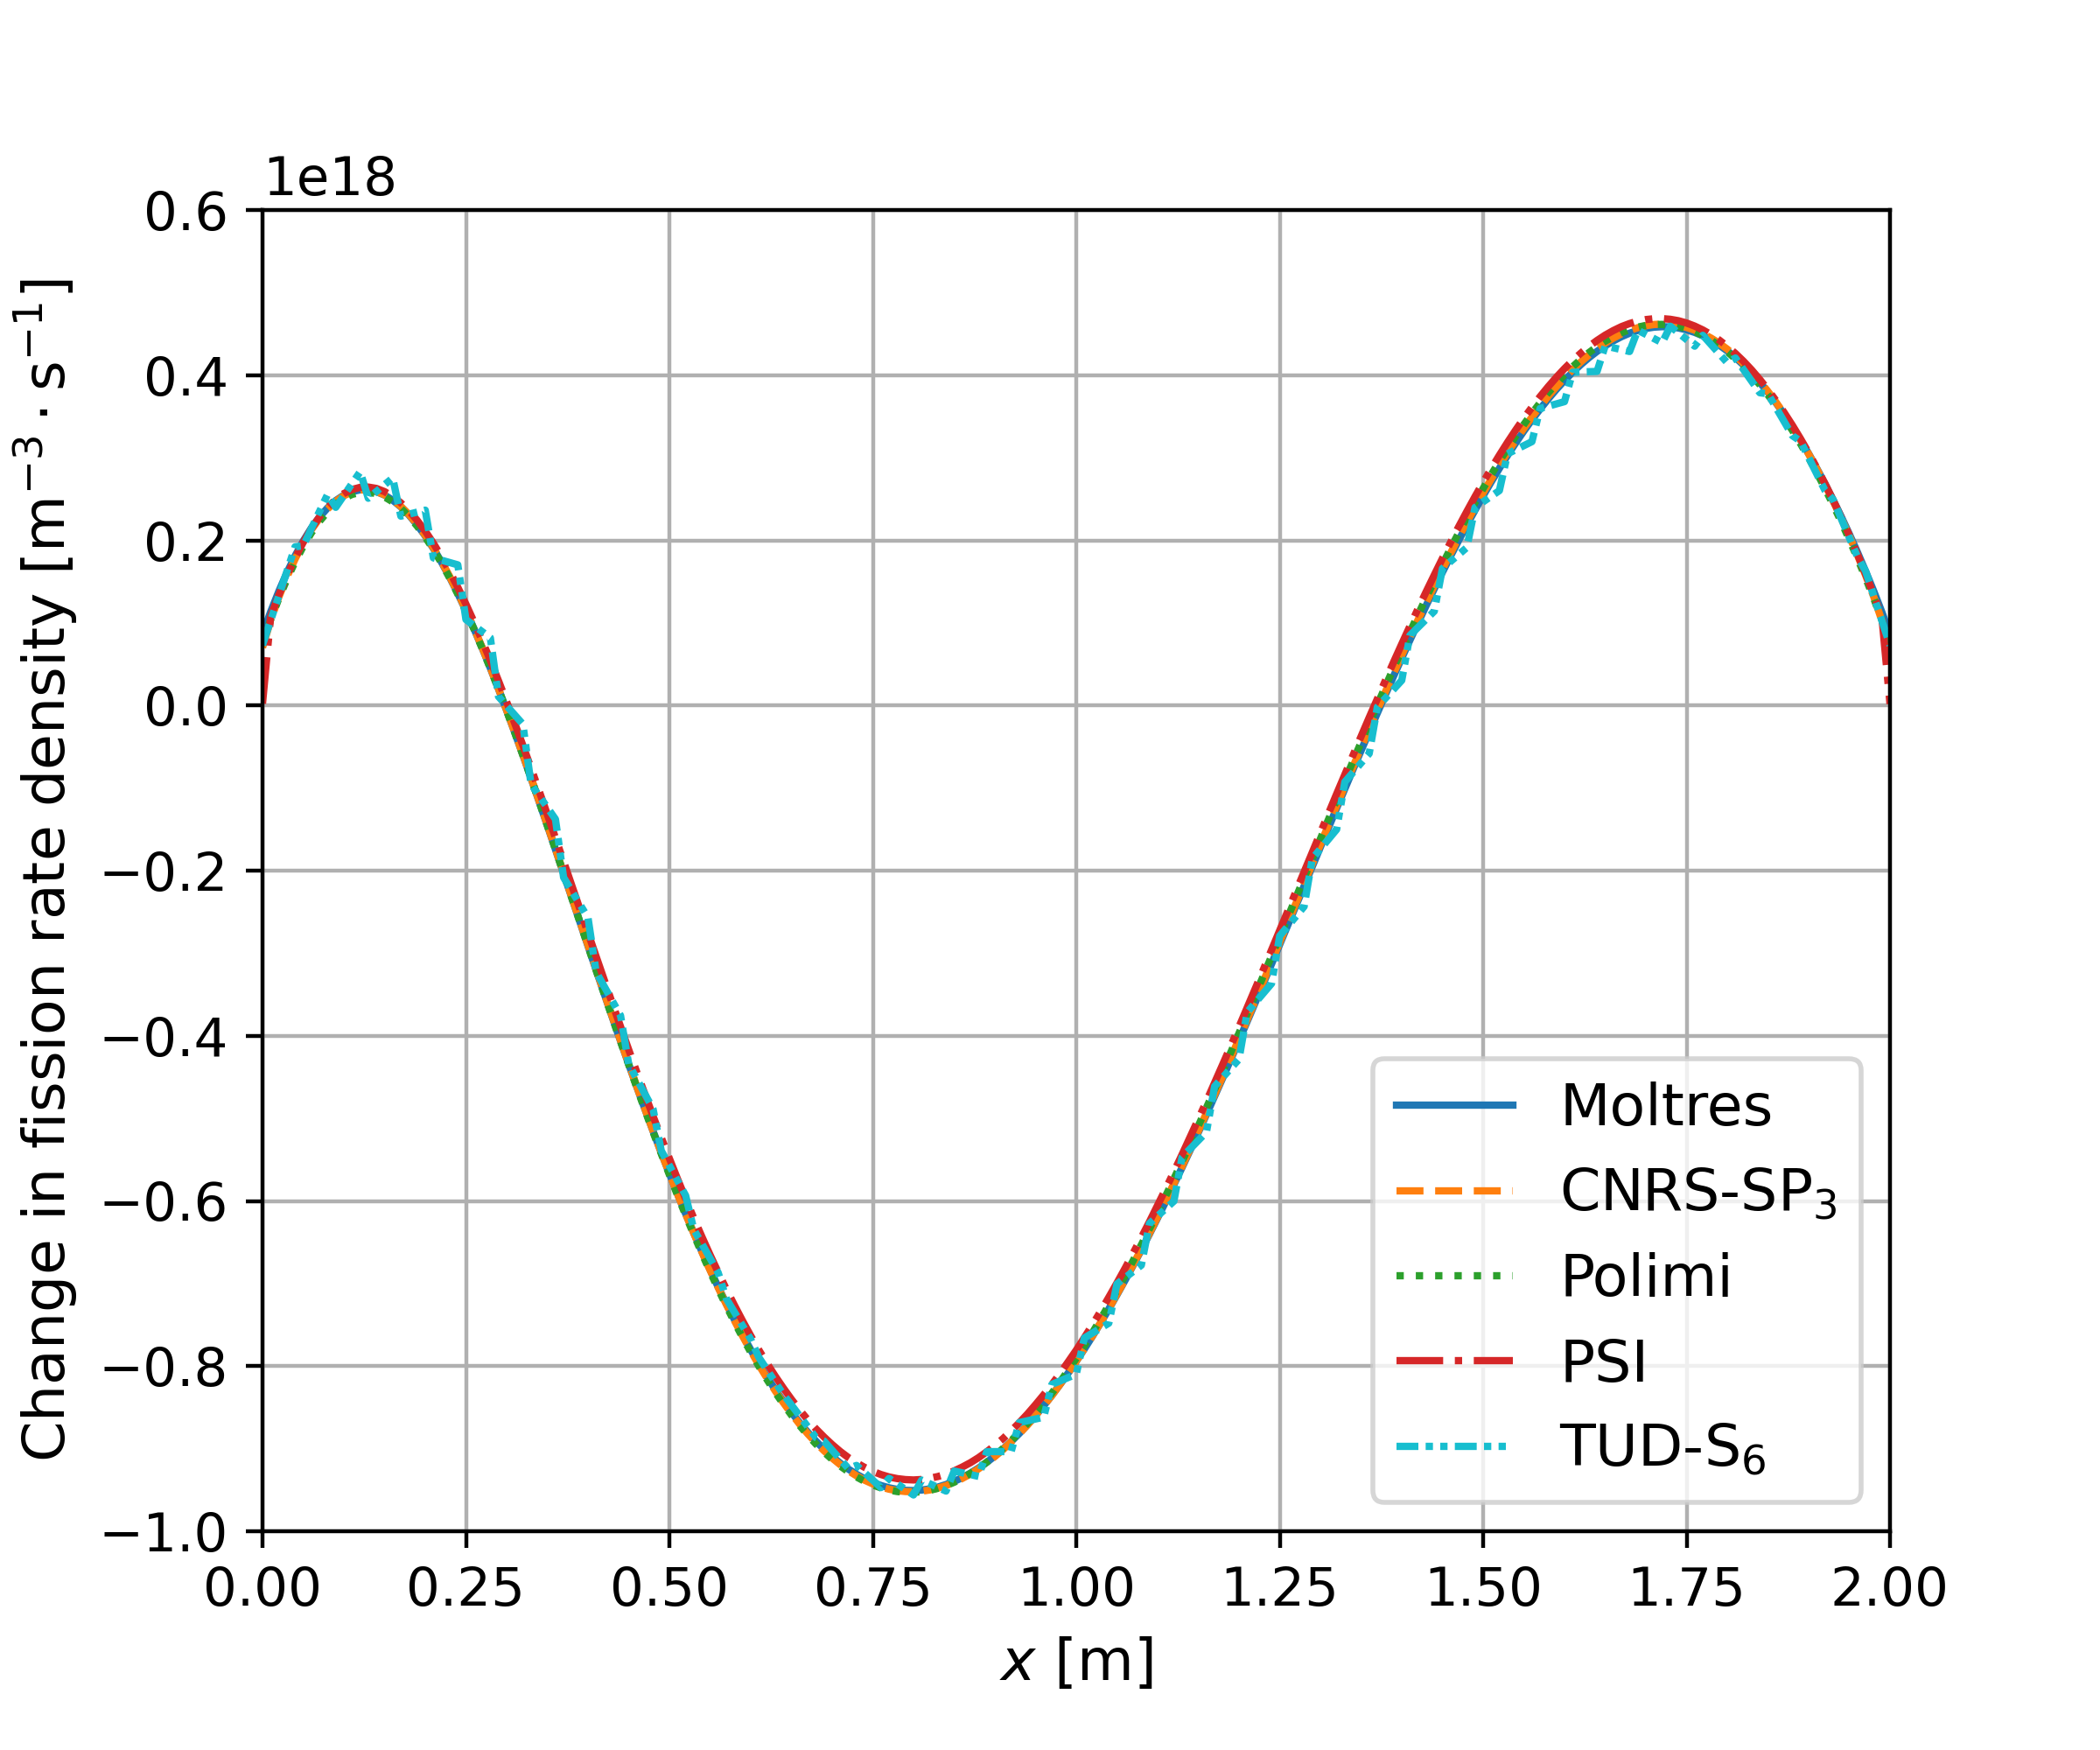
\includegraphics[width=.49\columnwidth]{1-2-fiss-plot}
	\caption{Step 1.2 \textemdash\ Temperature distribution and change in fission rate
	density along AA'.}
	\label{fig:1.2}
\end{figure}

\FloatBarrier

\paragraph{Step 1.2: Power coupling}

Figure \ref{fig:1.2} shows the temperature distribution and the change in
fission rate density along AA' from Step 1.2. Similar to Step 0.3, the
temperature distribution from Moltres agrees closest with CNRS-$SP_3$ and
TUD-$S_2$. Table \ref{table:disc1} reports the same trends we observed in Phase
0; the average discrepancy in temperature along BB' from Moltres for Step 1.2
is marginally higher than the benchmark, while the average discrepancy in the
fission rate density is within one \gls{SD} range to the benchmark average.
From Table \ref{table:rho}, Moltres also reports a change in $\rho$
relative to Step 1.1 of $-1142.2$ pcm, which
falls within the range of reported benchmark participants' values.

\paragraph{Step 1.3: Buoyancy}

Figure \ref{fig:1.3} shows the vertical velocity component, temperature, and
delayed neutron source distributions along AA'.
Moltres reproduces the correct trend in all three physical
observables. Step 1.3 has a relatively slower buoyancy-driven flow profile with
no forced flow from the top boundary. Consequently, there are no temperature
deviations near the top boundary, and we observe in Table \ref{table:disc1} that
the average discrepancy value of 0.070\% for the temperature distribution along
BB' is in much closer agreement to the benchmark value of 0.080\% compared to
the corresponding temperature discrepancy values for Step 0.3 and 1.2.

Table \ref{table:rho} shows that the change in $\rho$ from
Moltres (-1207.7 pcm) falls within the range of reported benchmark values and
matches the software from TUD-$S_2$ (-1208.5 pcm) the closest. This observation is likely
due to the similar solvers (diffusion and $S_2$ neutronics models) and
methods of solution (finite element method on uniform meshes) employed by our
respective software.
%
\begin{figure}[htb]
	\centering
	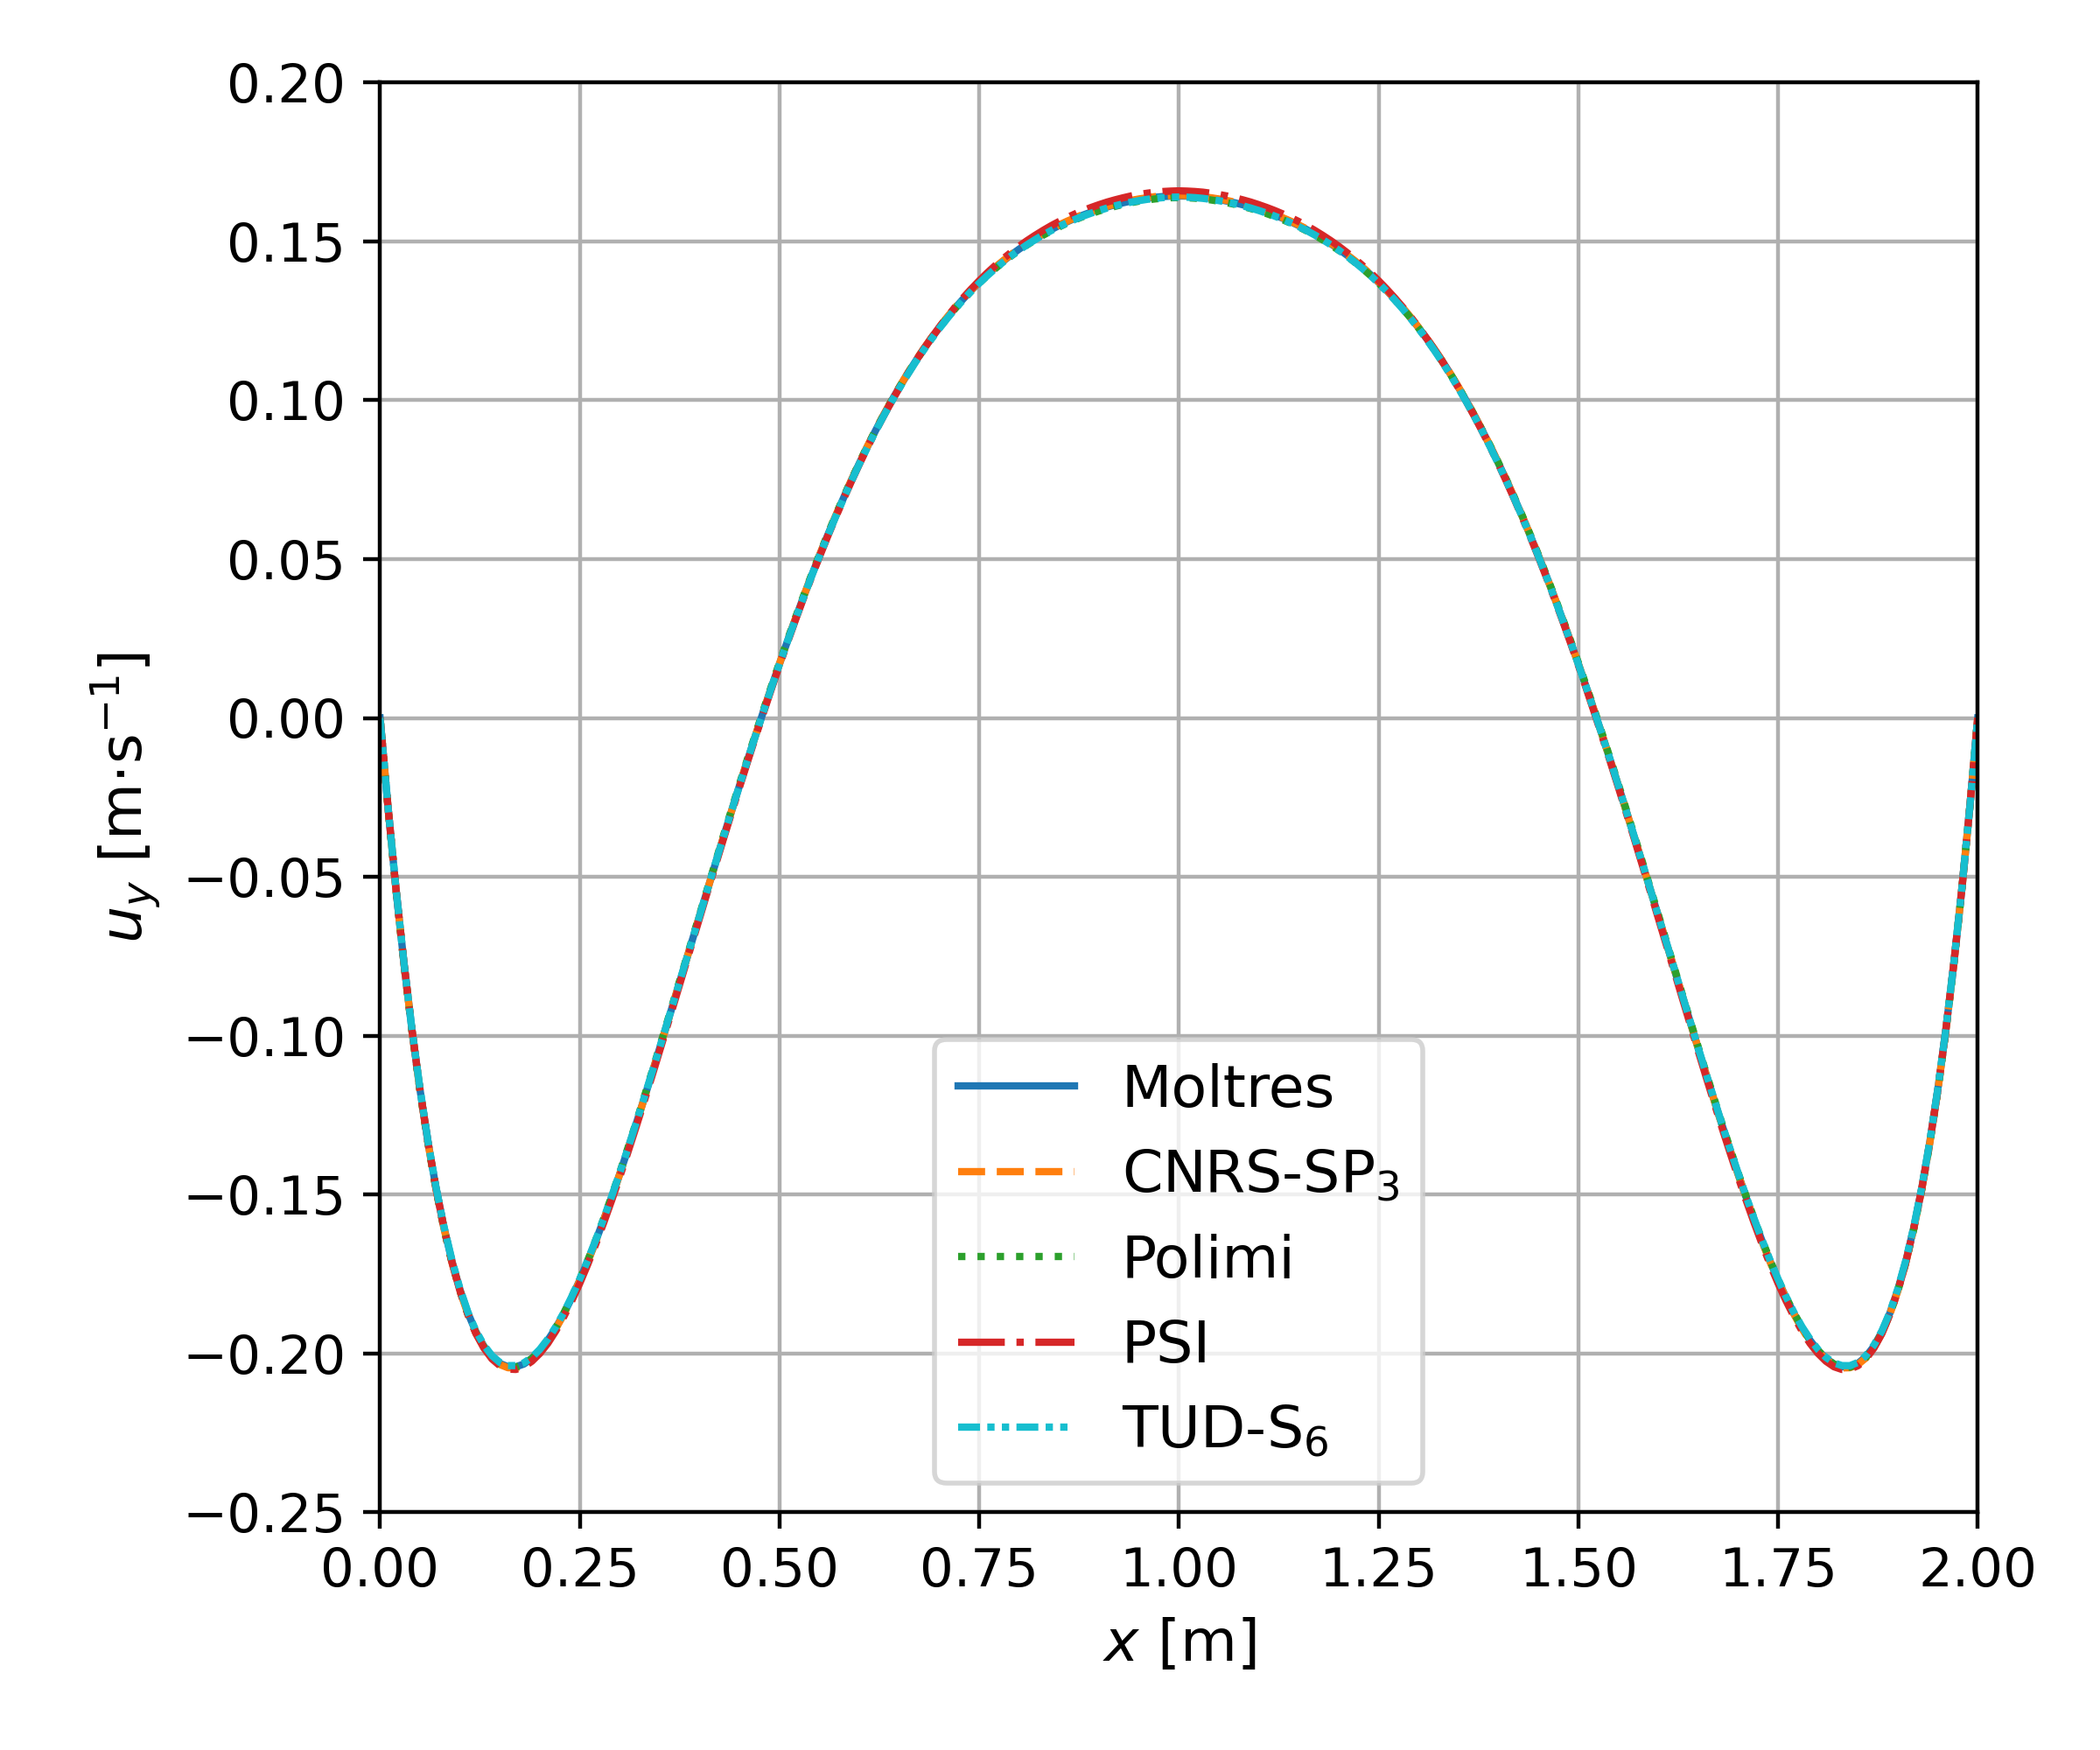
\includegraphics[width=.49\columnwidth]{1-3-vel-plot}
	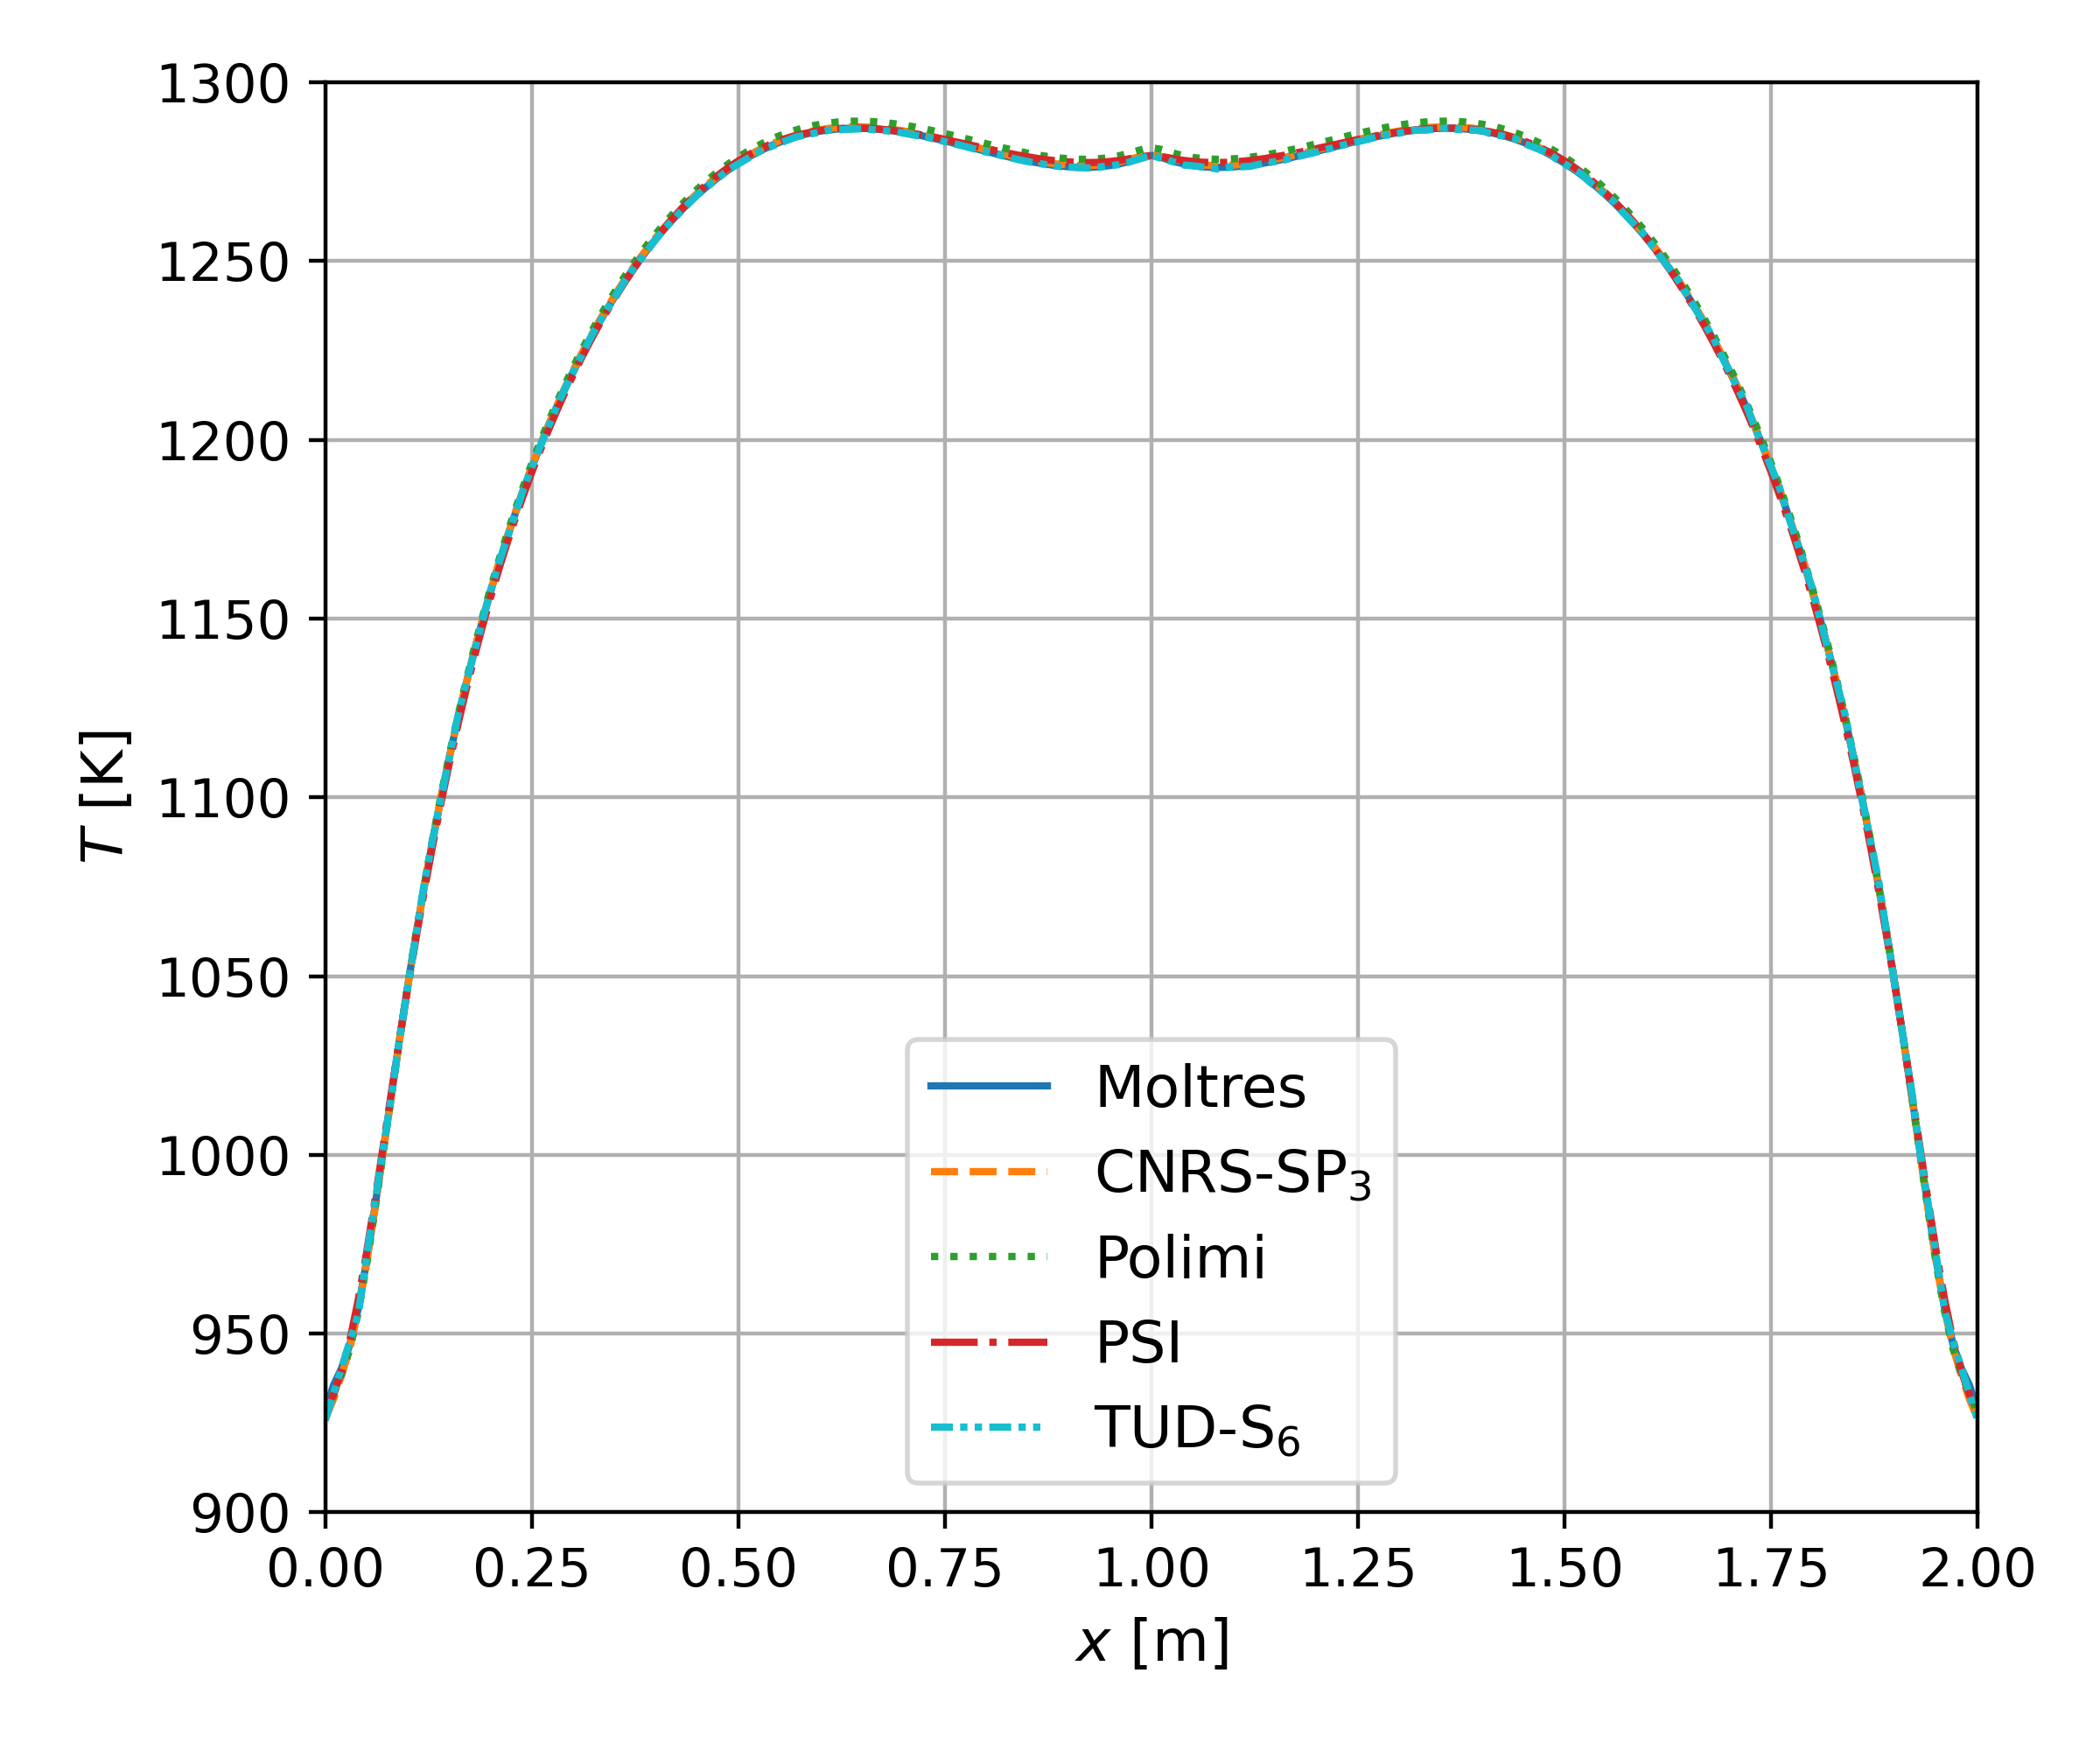
\includegraphics[width=.49\columnwidth]{1-3-temp-plot}
	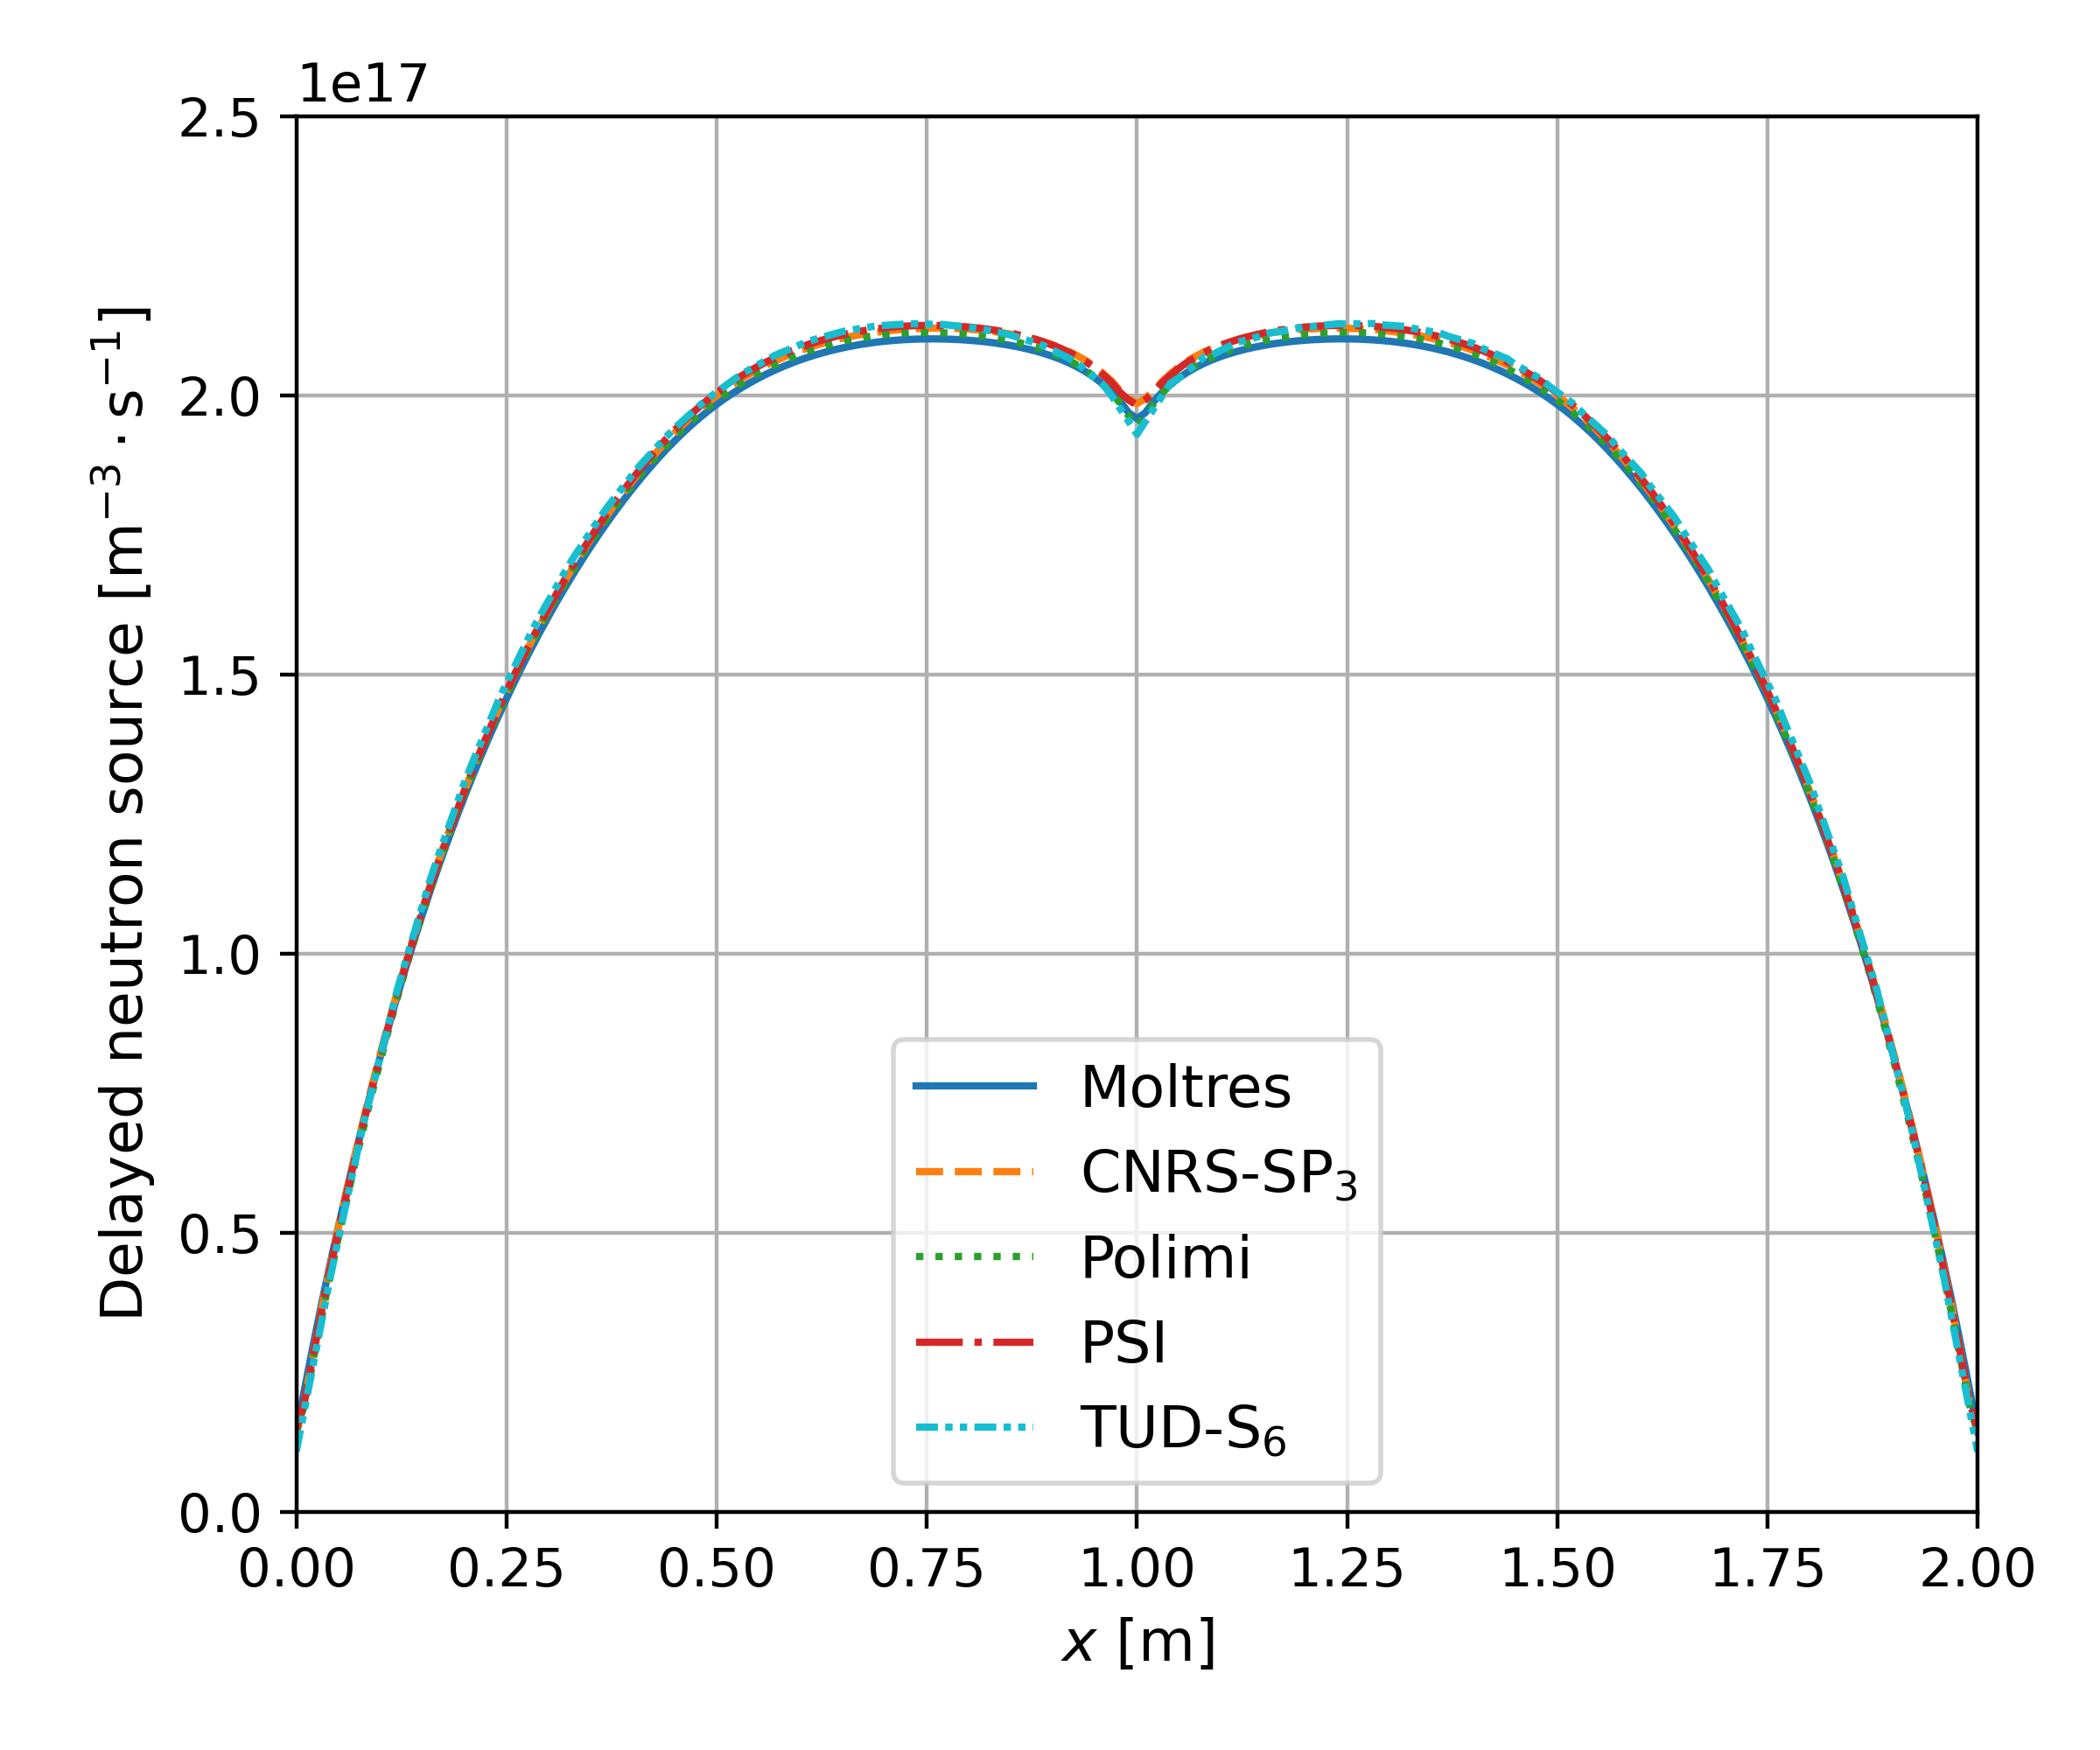
\includegraphics[width=.49\columnwidth]{1-3-dnp-plot}
	\caption{Step 1.3 \textemdash\ Vertical velocity component, temperature distribution,
	and delayed neutron source along AA'.}
	\label{fig:1.3}
\end{figure}

\FloatBarrier

\paragraph{Step 1.4: Full coupling}

Figure \ref{fig:cnrs-color} shows 2D temperature distribution and velocity
streamlines from Moltres for Step 1.4 with $U_{lid} = 0.5$ m$\cdot$s$^{-1}$ and
$P = 1$ GW. Table \ref{table:full} shows the change in $\rho$ under the various
$U_{lid}$ and $P$ values. Refer to Tiberga et al.'s paper
\cite{tiberga_results_2020} for the benchmark participants' corresponding
values. The change in $\rho$ values from Moltres all fall within the range of
benchmark values
for all cases. Furthermore, the $\Delta\rho$ values are all within 1.1 pcm of
the corresponding values from the TUD-S$_2$ model in the benchmark paper. Given
that the $S_2$ discrete ordinates method with isotropic sources is theoretically equivalent to the
multigroup neutron diffusion method, Moltres is largely
consistent with the benchmark participants outside of differences from the
neutronics models.

\begin{figure}[htb]
  \centering
  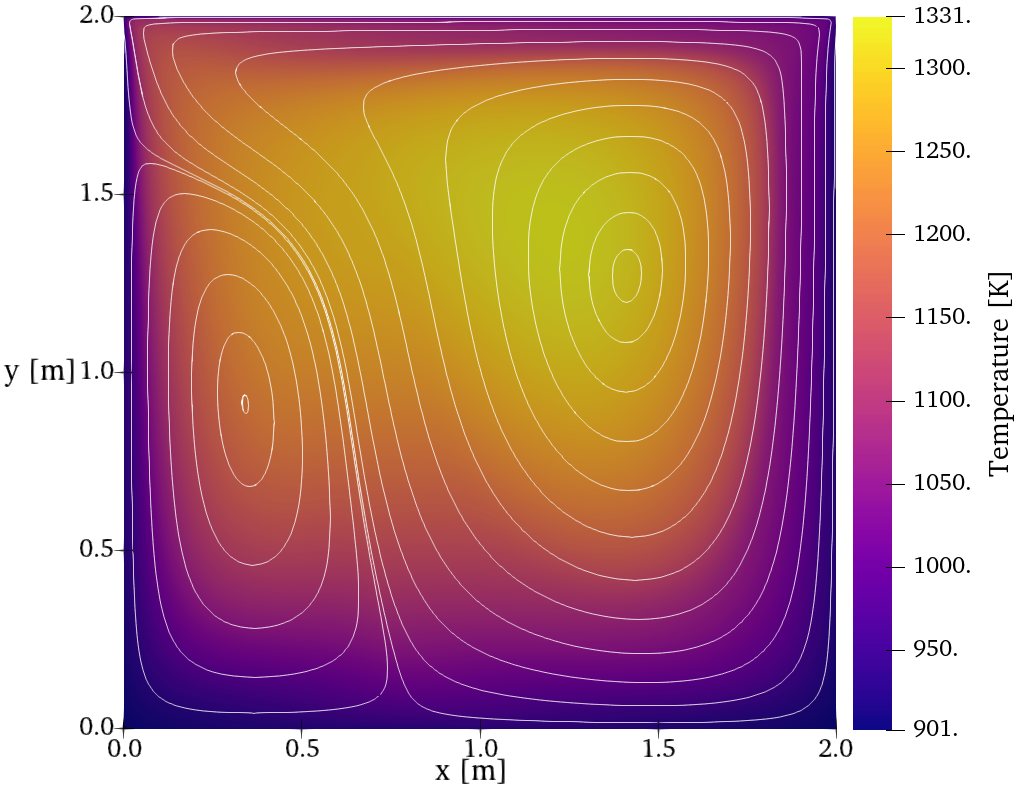
\includegraphics[width=.7\columnwidth]{full-coupled}
  \caption{Temperature distribution from Moltres for the fully coupled
  system (Step 1.4) with buoyancy effects, $P = 1$ GW, and $U_{lid} = 0.5$
  m$\cdot$s$^{-1}$. The lines correspond to the streamlines of the velocity
  field.}
  \label{fig:cnrs-color}
\end{figure}
%
\begin{table}[htb]
	\caption{Reactivity change in Step 1.4, relative to Step 0.2 under various
	$U_{lid}$ and $P$ values.}
	\centering
	\small
	\setlength\tabcolsep{1.5pt}
	\begin{tabular}{c c c c c c}
		\toprule
		& \multicolumn{5}{c}{$\rho_{s1.4} - \rho_{s0.2}$ [pcm]} \\
		\midrule
		{\backslashbox{$U_{lid}$ [m$\cdot$s$^{-1}$]}{$P$ [GW]}} & 0.2 & 0.4 & 0.6 & 0.8 & 1.0 \\
		\midrule
		0.0 & -263.7 & -498.3 & -730.9 & -966.7 & -1207.7 \\
		0.1 & -265.9 & -498.7 & -730.6 & -966.0 & -1206.7 \\
		0.2 & -268.1 & -498.8 & -729.4 & -963.7 & -1203.6 \\
		0.3 & -269.9 & -498.5 & -727.8 & -960.8 & -1199.5 \\
		0.4 & -271.9 & -498.5 & -726.5 & -958.3 & -1195.7 \\
		0.5 & -274.2 & -498.7 & -725.6 & -956.4 & -1192.7 \\
		\bottomrule
	\end{tabular}
	\label{table:full}
\end{table}

\FloatBarrier

\begin{table}[htb]
	\caption{Discrepancy values from Moltres alongside the average and standard
	deviation of the discrepancy values of the benchmark participants for Step
	2.1.}
	\centering
	\small
	\begin{tabular}{l l S S S}
		\toprule
		\multirow{2}{*}{\textbf{Step}} & \multirow{2}{*}{\textbf{Observable}} & {\multirow{2}{*}{\textbf{Moltres [\%]}}} & \multicolumn{2}{c}{\textbf{Benchmark [\%]}} \\
		& & & {Average} & {SD} \\
		\midrule
		\multirow{2}{*}{2.1} & Gain & 0.493 & 0.587 & 0.244 \\
		\cmidrule{2-5}
		& Phase shift & 1.741 & 2.176 & 0.554 \\
		\bottomrule
	\end{tabular}
	\label{table:disc2}
\end{table}
%
\begin{figure}[htb]
	\centering
	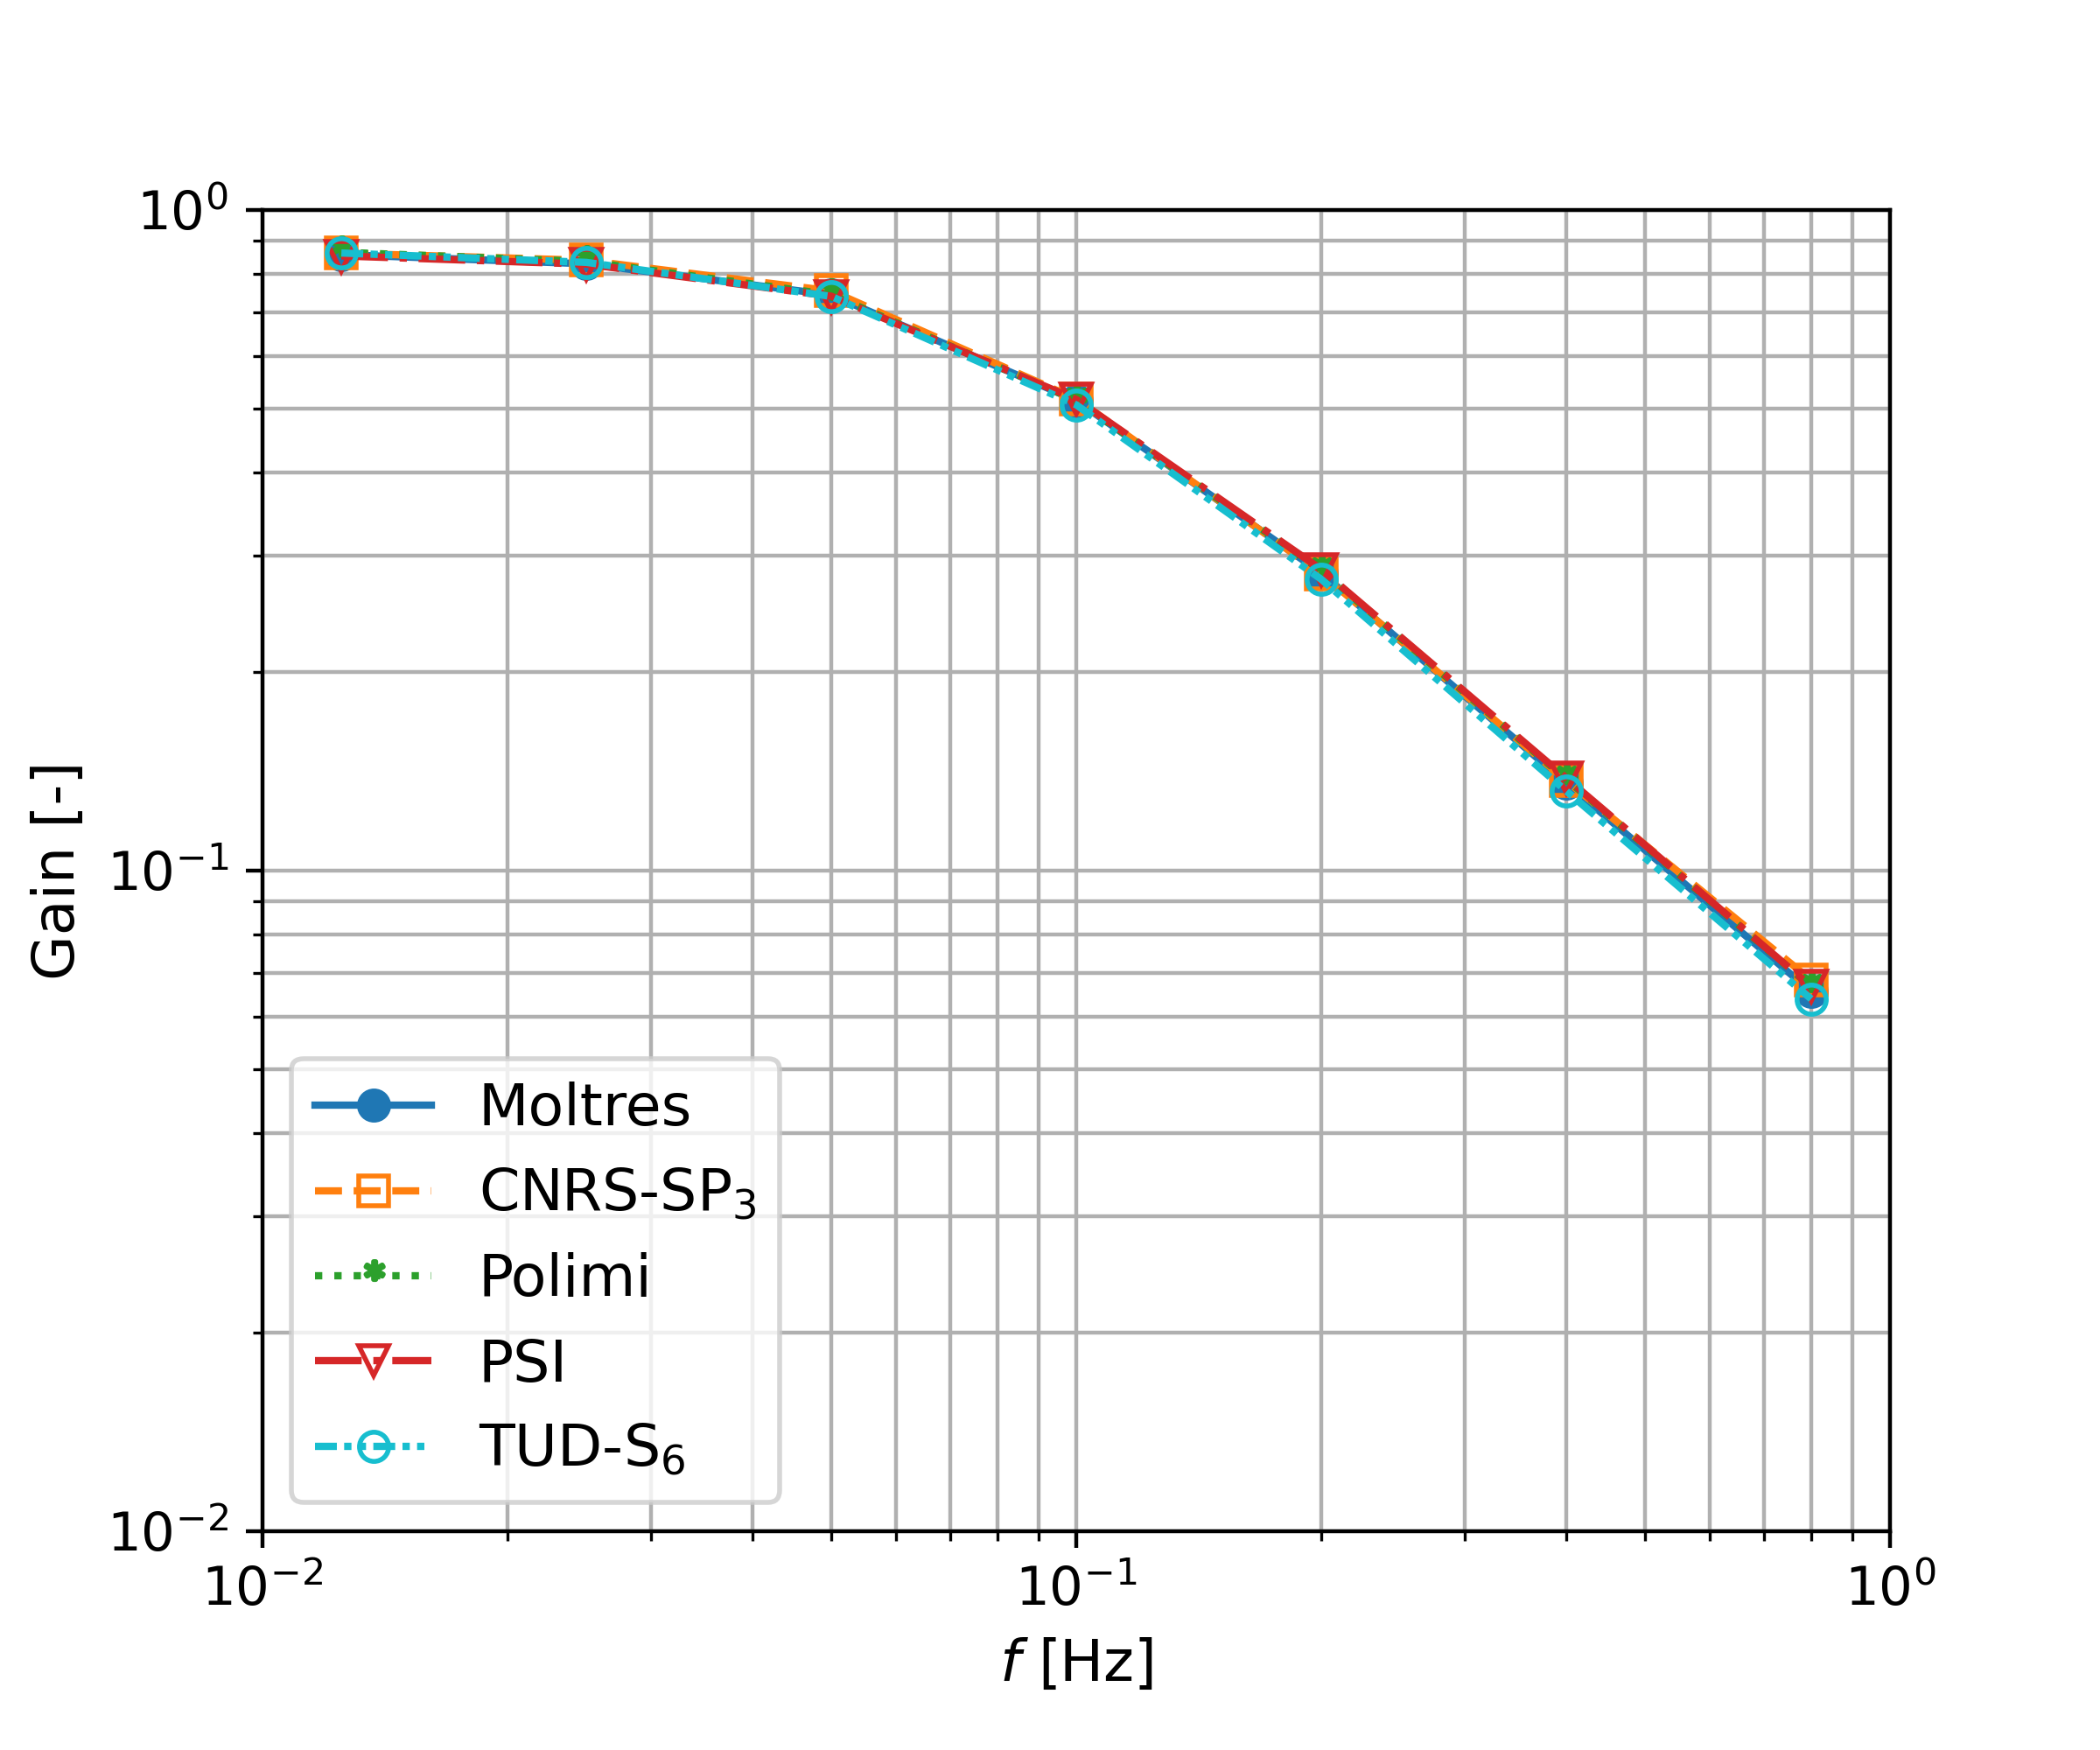
\includegraphics[width=.49\columnwidth]{2-1-gain-plot}
	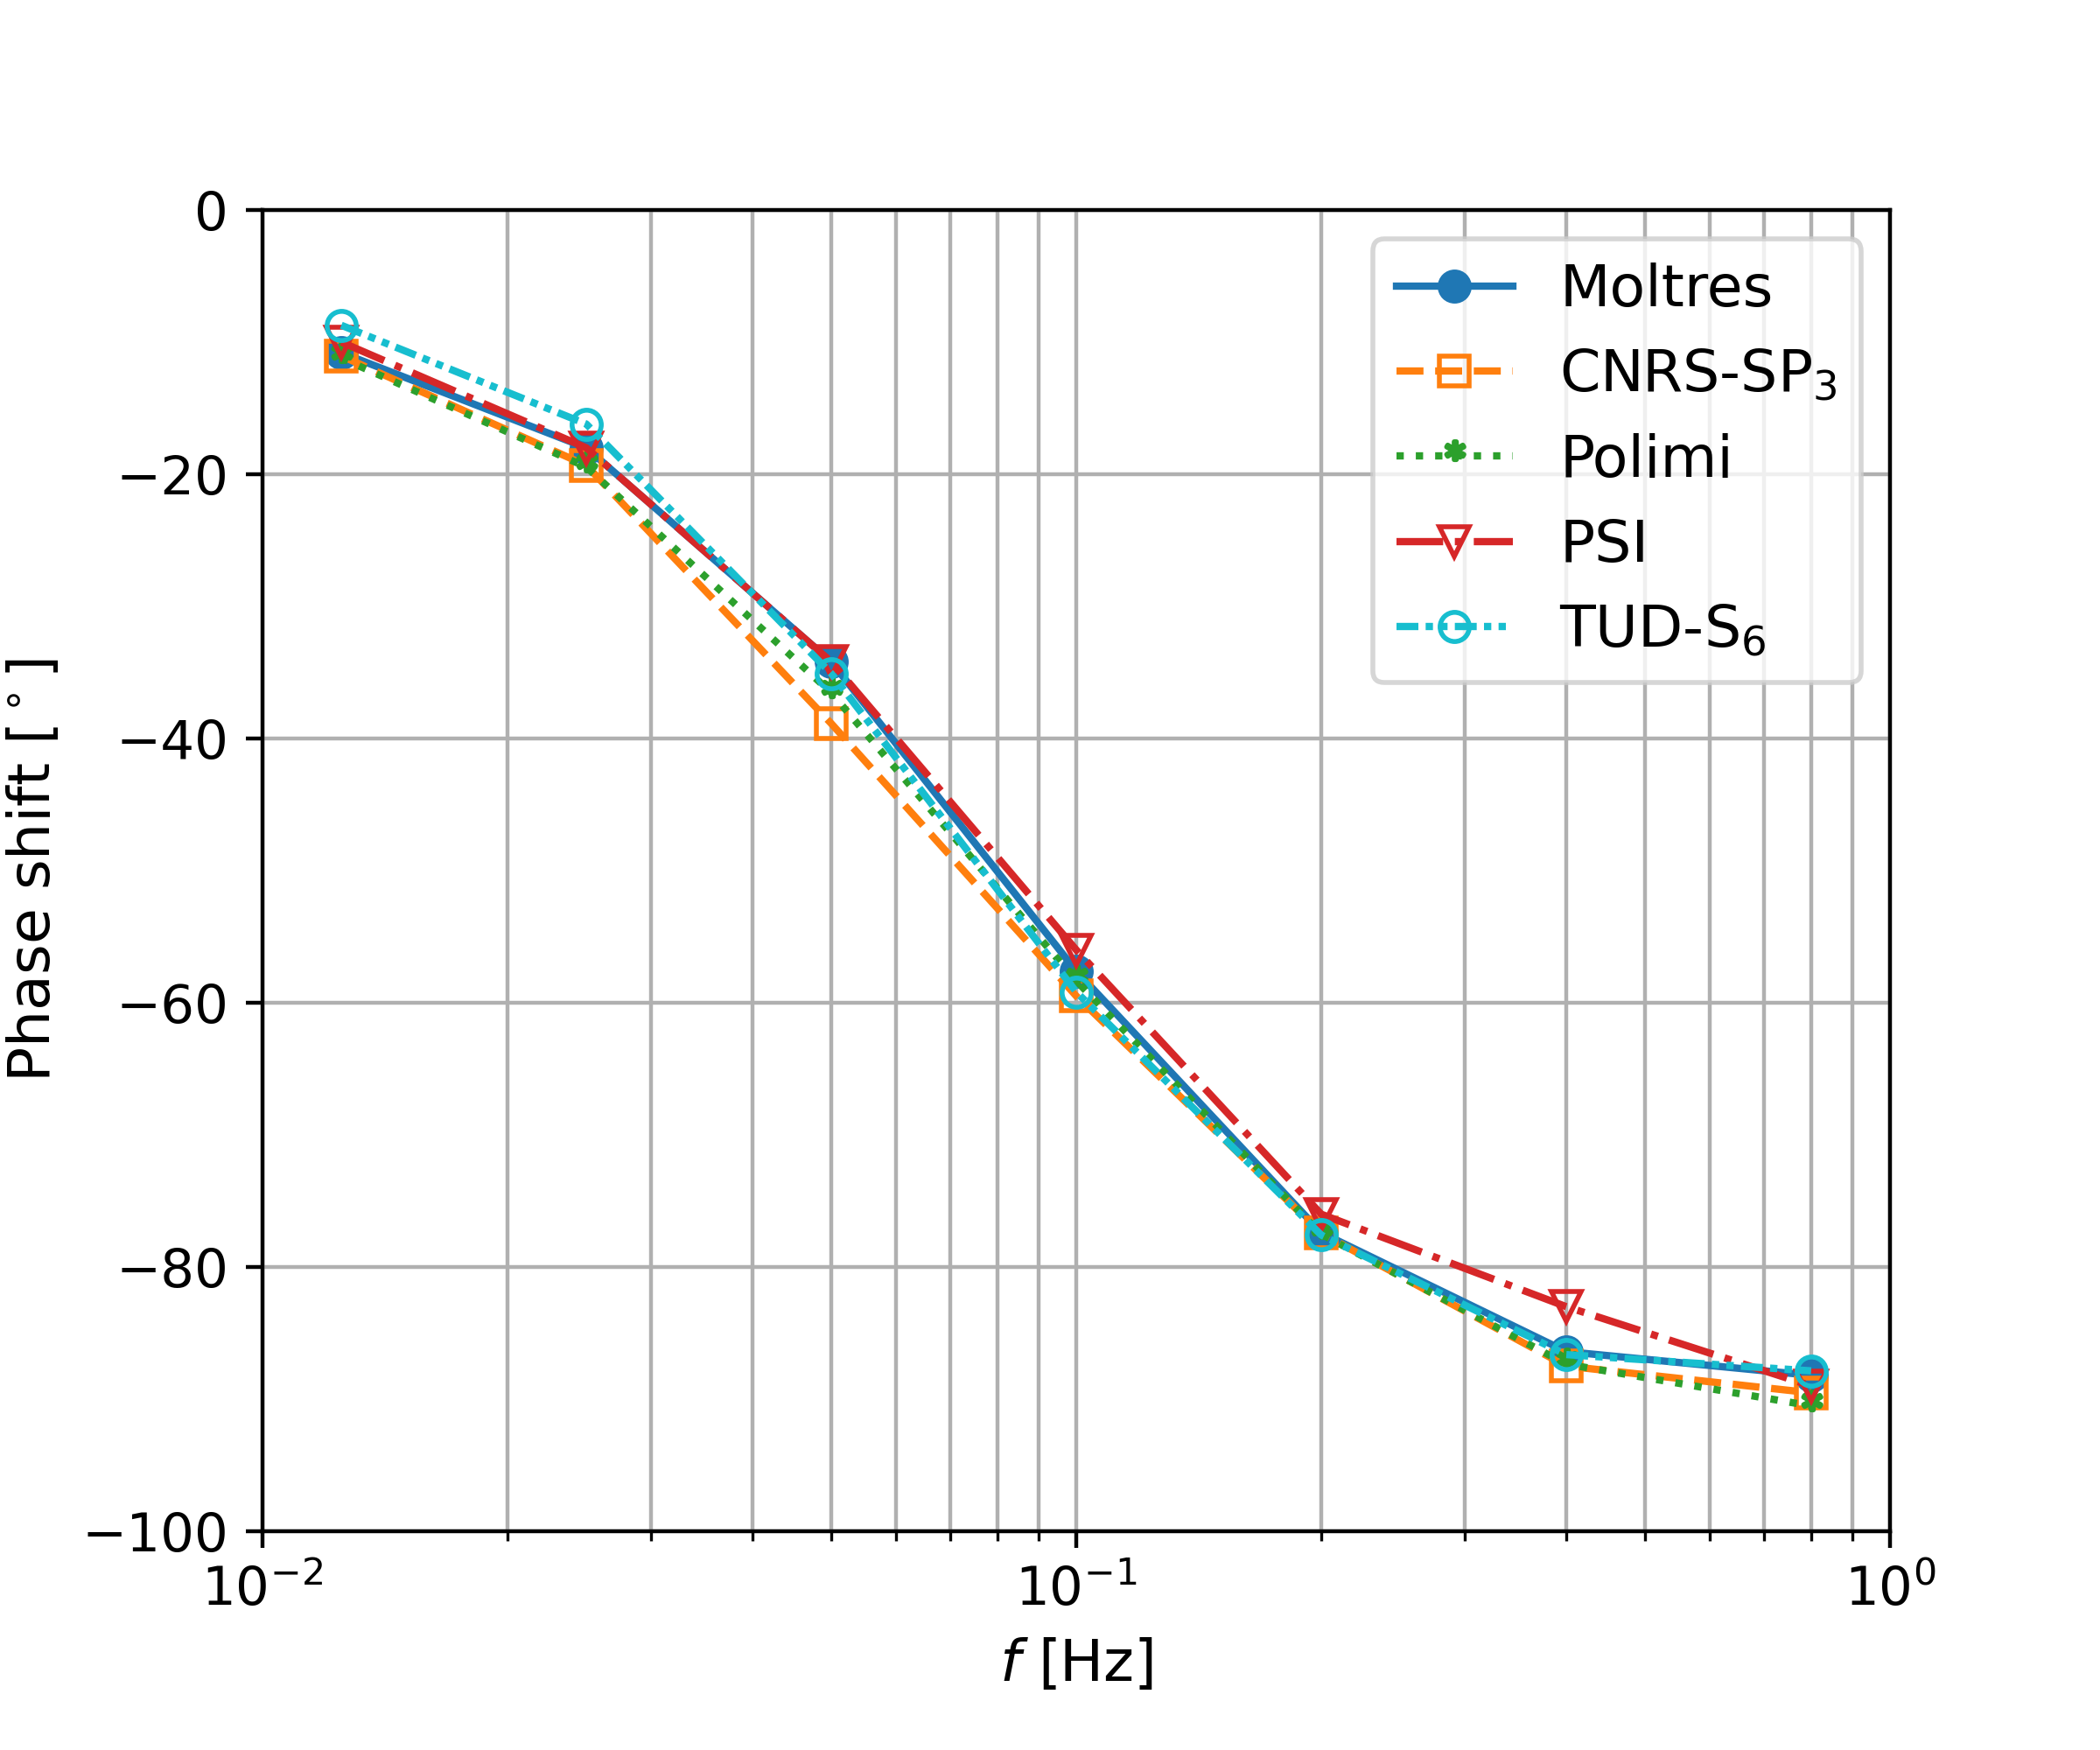
\includegraphics[width=.49\columnwidth]{2-1-phase-plot}
	\caption{Step 2.1 \textemdash\ Bode gain and phase plots of the frequency response of
	the fully coupled system.}
	\label{fig:2.1}
\end{figure}

\subsubsection{Phase 2 results \& discussion}

Lastly, the following subsection discusses the results for the transient cases
in Step 2.1, which involve measuring the response in power output to periodic
perturbations in the heat transfer coefficient.

\paragraph{Step 2.1: Forced convection transient}

Figure \ref{fig:2.1} shows the Bode gain and phase shift plots of the response
in power output in the fully coupled system. Along with the average discrepancy
values from Table \ref{table:disc2}, the results show that Moltres is
consistent with the benchmark. The gain data points from all \gls{MSR} software
agree closely with one another. Moltres reports an average discrepancy value of
0.496\%, slightly lower than the benchmark average of 0.587\%. On the other
hand, the phase shift data points show a greater spread over the various driving
frequencies. We note the different timestepping schemes and timestep
sizes among the different software packages, which is likely responsible for
the variations in the phase shift. Even with a precision of
$\pm0.9^\circ$ for each phase shift value, Moltres accurately reproduces the
correct trend with a lower average discrepancy (1.741\%) than the benchmark
participants' average (2.176\%).

\FloatBarrier
